\documentclass[twoside]{article}

\usepackage{aistats2023}
% If your paper is accepted, change the options for the package
% aistats2023 as follows:
%
% \usepackage[accepted]{aistats2023}
%
% This option will print headings for the title of your paper and
% headings for the authors names, plus a copyright note at the end of
% the first column of the first page.

% If you set papersize explicitly, activate the following three lines:
%\special{papersize = 8.5in, 11in}
%\setlength{\pdfpageheight}{11in}
%\setlength{\pdfpagewidth}{8.5in}

% If you use natbib package, activate the following three lines:
%\usepackage[round]{natbib}
%\renewcommand{\bibname}{References}
%\renewcommand{\bibsection}{\subsubsection*{\bibname}}

% If you use BibTeX in apalike style, activate the following line:
%\bibliographystyle{apalike}

\usepackage[utf8]{inputenc} % allow utf-8 input
\usepackage[T1]{fontenc}    % use 8-bit T1 fonts
\usepackage{hyperref}       % hyperlinks
\usepackage{url}            % simple URL typesetting
\usepackage{booktabs}       % professional-quality tables
\usepackage{amsfonts}       % blackboard math symbols
\usepackage{nicefrac}       % compact symbols for 1/2, etc.
\usepackage{microtype}      % microtypography
\usepackage{xcolor}         % colors
\usepackage{enumitem}


%\usepackage{charter}
%\usepackage{calc}

\usepackage{multirow}
% \usepackage[cp1250]{inputenc}
% \usepackage[T1]{fontenc}
% \usepackage{calligra}
\usepackage{layout}

% AMS
\usepackage{amsmath}
\usepackage{amsthm}
\usepackage{amssymb}
\usepackage{amsfonts}
\usepackage{mathtools}
\usepackage{siunitx}

\usepackage{bbm}

\usepackage{url}
\usepackage{color}
\usepackage{graphicx}
\usepackage{algorithmic}
\usepackage{algorithm}
\usepackage{verbatim}

\usepackage{apptools}
\usepackage{thmtools}
% \usepackage{algpseudocode}

% paper specific macros
\newcommand{\g}{{\color{red}g}}
\newcommand{\h}{{\color{blue}h}}

% general macros

\newcommand{\norm}[1]{\left\| #1 \right\|}
\newcommand{\sqnorm}[1]{\left\| #1 \right\|^2}
\newcommand{\lin}[1]{\left\langle #1\right\rangle} % inner product
\newcommand{\inp}[2]{\left\langle#1,#2\right\rangle} % inner product

% caligraphic
\newcommand{\cA}{\mathcal{A}}
\newcommand{\cB}{\mathcal{B}}
\newcommand{\cC}{\mathcal{C}}
\newcommand{\cD}{\mathcal{D}}
\newcommand{\cH}{\mathcal{H}}
\newcommand{\cL}{\mathcal{L}}
\newcommand{\cO}{\mathcal{O}}
\newcommand{\cQ}{\mathcal{Q}}
\newcommand{\cS}{\mathcal{S}}
\newcommand{\cW}{\mathcal{W}}
\newcommand{\cY}{\mathcal{Y}}
\newcommand{\cZ}{\mathcal{Z}}

% bold matrices
\newcommand{\mM}{\mathbf{M}}
\newcommand{\mN}{\mathbf{N}}
\newcommand{\mI}{\mathbf{I}}
\newcommand{\mJ}{\mathbf{J}}
\newcommand{\mL}{\mathbf{L}}
\newcommand{\mD}{\mathbf{D}}
\newcommand{\mO}{\mathbf{O}}


% strange stuff
\newcommand{\hotidea}{{\color{red}\bf HOT IDEA: }}
\newcommand{\done}{{\color{blue}\bf DONE: }}
\newcommand{\del}[1]{}
\let\la=\langle
\let\ra=\rangle

% basic macros
\newcommand{\R}{\mathbb{R}} % reals
\newcommand{\U}{\mathbb{U}} % reals
\newcommand{\PermComp}{\U\mathbb{P}} % reals

\newcommand{\st}{\;:\;} % such that
%\newcommand{\eqdef}{\stackrel{\text{def}}{=}}
\newcommand{\eqdef}{:=} %\vcentcolon

\newcommand{\Prob}{\mathbf{Prob}} % probability
\newcommand{\ProbCond}[2]{\Prob\left(\left.#1\right\vert#2\right)}

\newcommand{\nnz}[1]{{\color{red}\|#1\|_0}}

% sets
\DeclareMathOperator{\card}{card}         % cardinality of a set
\DeclareMathOperator{\diam}{diam}        % diameter of a set
\DeclareMathOperator{\vol}{vol}               % volume of a set

% statistics
\newcommand{\Exp}[1]{{\rm E}\left[#1\right]}
\newcommand{\ExpCond}[2]{{\rm E}\left[\left.#1\right\vert#2\right]}
\newcommand{\ExpSub}[2]{{\rm E}_{#1}\left[#2\right]}
\DeclareMathOperator{\Cov}{Cov}         % covariance
\DeclareMathOperator{\Var}{Var}         % variance
\DeclareMathOperator{\Corr}{Corr}       % correlation

% functions and operators
\DeclareMathOperator{\signum}{sign}     % signum/sign of a scalar
\DeclareMathOperator{\dom}{dom}         % domain
\DeclareMathOperator{\epi}{epi}         % epigraph
\DeclareMathOperator{\Ker}{null}        % nullspace/kernel
\DeclareMathOperator{\nullspace}{null}  % nullpsace
\DeclareMathOperator{\range}{range}     % range
\DeclareMathOperator{\Image}{Im}        % image

% topology
\DeclareMathOperator{\interior}{int}    % interior
\DeclareMathOperator{\ri}{rint}         % relative interior
\DeclareMathOperator{\rint}{rint}       % relative interior
\DeclareMathOperator{\bdry}{bdry}       % boundary
\DeclareMathOperator{\cl}{cl}           % closure

% vectors, matrices
\DeclareMathOperator{\linspan}{span}
\DeclareMathOperator{\linspace}{linspace}
\DeclareMathOperator{\cone}{cone}

\DeclareMathOperator{\tr}{tr}           % trace
\DeclareMathOperator{\rank}{rank}       % rank
\DeclareMathOperator{\conv}{conv}       % convex hull
\DeclareMathOperator{\Diag}{Diag}       % Diag(v) = diagonal matrix with v_i on the diagonal
\DeclareMathOperator{\diag}{diag}       % diag(D) = the diagonal vector of matrix D
\DeclareMathOperator{\Arg}{Arg}         % Argument

%\renewcommand{\qedsymbol}{\ding{114}}




%%%%%%%%

% TODO: Fix here fonts
\newcommand{\Sample}{\mathcal{S}}
%\newcommand{\E}{\mathbb{E}}
%\newcommand{\norm}[1]{\left\lVert#1\right\rVert_2}
\newcommand{\B}{\mathbb{B}}


\usepackage{tcolorbox}
\usepackage{pifont}
\definecolor{mydarkgreen}{RGB}{39,130,67}
\definecolor{mydarkred}{RGB}{192,47,25}
\newcommand{\green}{\color{mydarkgreen}}
\newcommand{\red}{\color{mydarkred}}
\newcommand{\cmark}{\green\ding{51}}%
\newcommand{\xmark}{\red\ding{55}}%

\newcommand{\algname}[1]{{\green\small \sf #1}}
\newcommand{\algnamesmall}[1]{{\green\scriptsize \sf #1}}

\newcommand{\tablescriptsize}[1]{{\scriptsize #1}}
\newcommand{\tablesmall}[1]{{\small #1}}



%%%%%%%%

\newtheorem{assumption}{Assumption}
\newtheorem{lemma}{Lemma}
\newtheorem{algorithms}{Algorithm}
\newtheorem{theorem}{Theorem}
\newtheorem{proposition}{Proposition}
\newtheorem{example}{Example}
\newtheorem{corollary}{Corollary}

\theoremstyle{plain}

\newtheorem{prop}[theorem]{Proposition}
\newtheorem{cor}[theorem]{Corollary}
\newtheorem{lem}[theorem]{Lemma}
\newtheorem{claim}[theorem]{Claim}
\newtheorem{remark}[theorem]{Remark}

\theoremstyle{definition}

\newtheorem{exercise}[theorem]{Exercise}

\newtheorem{rem}[theorem]{Remark}
\newtheorem{que}[theorem]{Question}
\newtheorem{definition}[theorem]{Definition}

% Hack that enables labeling of lines in algorithms
\newcommand{\alglinelabel}{%
  \addtocounter{ALC@line}{-1}% Reduce line counter by 1
  \refstepcounter{ALC@line}% Increment line counter with reference capability
  \label% Regular \label
}
\usepackage[textsize=tiny]{todonotes}
\usepackage{footnote}
\usepackage{mathtools}
\usepackage[flushleft]{threeparttable}
\usepackage{etoolbox}

\usepackage{natbib}

\newcommand{\alexander}[1]{\todo[inline]{\textbf{Alexander: }#1}}

\newcommand{\algorithmname}{DASHA-PP}

\newcommand*{\probavailable}{\ensuremath{p_{\textnormal{a}}}}
\newcommand*{\probpairaa}{\ensuremath{p_{\textnormal{aa}}}}
\newcommand*{\probpairan}{\ensuremath{p_{\textnormal{an}}}}
\newcommand*{\probpairnn}{\ensuremath{p_{\textnormal{nn}}}}

\newcommand*{\probpage}{\ensuremath{p_{\text{page}}}}
\newcommand*{\probmega}{\ensuremath{p_{\text{mega}}}}

\allowdisplaybreaks
\makeatletter
\newcommand{\vast}{\bBigg@{4}}
\newcommand{\Vast}{\bBigg@{5}}
\makeatother

\newcommand{\improvement}[1]{{\color{orange}#1}}
\newcommand{\degeneration}[1]{{\color{red}#1}}

\hypersetup{
  colorlinks   = true, %Colours links instead of ugly boxes
  urlcolor     = blue, %Colour for external hyperlinks
  linkcolor    = {red!75!black}, %Colour of internal links
  citecolor   = {blue!50!black} %Colour of citations
}

\begin{document}

% If your paper is accepted and the title of your paper is very long,
% the style will print as headings an error message. Use the following
% command to supply a shorter title of your paper so that it can be
% used as headings.
%
%\runningtitle{I use this title instead because the last one was very long}

% If your paper is accepted and the number of authors is large, the
% style will print as headings an error message. Use the following
% command to supply a shorter version of the authors names so that
% they can be used as headings (for example, use only the surnames)
%
%\runningauthor{Surname 1, Surname 2, Surname 3, ...., Surname n}

\twocolumn[

\aistatstitle{A Computation and Communication Efficient Method \\ for Distributed Nonconvex Problems in the Partial Participation Setting}

\aistatsauthor{Alexander Tyurin 
\And
Peter Richt\'{a}rik}

\aistatsaddress{ KAUST, Saudi Arabia \And KAUST, Saudi Arabia } ]

\begin{abstract}
  We present a new method that includes three key components of distributed optimization and federated learning: variance reduction of stochastic gradients, compressed communication, and partial participation. We prove that the new method has optimal oracle complexity and state-of-the-art communication complexity in the partial participation setting. Moreover, we observe that "1 + 1 + 1 is not 3": by mixing variance reduction of stochastic gradients with compressed communication and partial participation, we do not obtain a fully synergetic effect. We explain the nature of this phenomenon, argue that this is to be expected, and propose possible workarounds.
\end{abstract}

\section{Introduction}
Federated and distributed learning have become very popular in recent years \citep{konevcny2016federated, mcmahan2017communication}. 
The current optimization tasks require much computational resources and machines. Such requirements emerge in machine learning, where massive datasets and computations are distributed between cluster nodes \citep{lin2017deep, ramesh2021zero}. In federated learning, nodes, represented by mobile phones, laptops, and desktops, do not send their data to a server due to privacy and their huge number \citep{ramaswamy2019federated}, and the server remotely orchestrates the nodes and communicates with them to solve an optimization problem.

As in classical optimization tasks, one of the main current challenges is to find \textbf{computationally efficient} optimization algorithms. However, the nature of distributed problems induces many other \citep{kairouz2021advances}, including i) \textbf{partial participation} of nodes in algorithm steps: due to stragglers \citep{li2020federated} or communication delays \citep{vogels2021relaysum}, ii) \textbf{communication bottleneck}: even if a node participates, it can be costly to transmit information to a server or other nodes \citep{alistarh2017qsgd, ramesh2021zero,kairouz2021advances, sapio2019scaling, narayanan2019pipedream}. It is necessary to develop a method that considers these problems.

% \begin{enumerate}
%   \item Partial Participation (No Synchronization)
%   \item Variance Reduction
%   \item Compression
% \end{enumerate}

\section{Optimization Problem}
\label{sec:opt_problem}
Let us consider the nonconvex distributed optimization problem
\begin{align}
    \label{eq:main_problem} 
    \min \limits_{x \in \R^d}\left\{f(x) \eqdef \frac{1}{n}\sum \limits_{i=1}^n f_i(x)\right\},
\end{align}
where $f_i\,:\,\R^d \rightarrow \R$ is a smooth nonconvex function for all $i \in [n] \eqdef \{1, \dots, n\}.$ The full information about function $f_i$ is stored on $i$\textsuperscript{th} node. The communication between nodes is maintained in the parameters server fashion \citep{kairouz2021advances}: we have a server that receives compressed information from nodes, updates a state, and broadcasts an updated model.\footnote{Note that this strategy can be used in peer-to-peer communication, assuming that the server is an abstraction and all its algorithmic steps are performed on each node.} Since we work in the nonconvex world, our goal is to find an $\varepsilon$-solution ($\varepsilon$-stationary point) of \eqref{eq:main_problem}: a (possibly random) point $\widehat{x}\in \R^d$, such that ${\rm E}\big[\norm{\nabla f(\widehat{x})}^2\big] \leq \varepsilon.$

We consider three settings:
\begin{enumerate}[leftmargin=0.75cm]
\item \textbf{Gradient Setting.}
The $i$\textsuperscript{th} node has only access to the gradient $\nabla f_i \,:\,\R^d \rightarrow \R^d$ of function $f_i$. Moreover, the following assumptions for the functions $f_i$ hold.
\begin{assumption}
    \label{ass:lower_bound}
    There exists $f^* \in \R$ such that $f(x) \geq f^*$ for all $x \in \R$.
\end{assumption}
\begin{assumption}
    \label{ass:lipschitz_constant}
    The function $f$ is $L$--smooth, i.e., $\norm{\nabla f(x) - \nabla f(y)} \leq L \norm{x - y}$ for all $x, y \in \R^d.$
\end{assumption}
\begin{assumption} \leavevmode
    \label{ass:nodes_lipschitz_constant}
    The functions $f_i$ are $L_i$--smooth for all $i \in [n]$. Let us define $\widehat{L}^2 \eqdef \frac{1}{n} \sum_{i=1}^{n} L_i^2.$\footnote{Note that $L \leq \widehat{L},$ $\widehat{L} \leq L_{\max},$ and $\widehat{L} \leq L_{\sigma}.$}
\end{assumption}

\item \textbf{Finite-Sum Setting.}
The functions $\{f_i\}_{i=1}^n$ have the finite-sum form
\begin{align}
    \label{eq:task_minibatch} f_i(x) = \frac{1}{n}\sum \limits_{j=1}^m f_{ij}(x), \qquad \forall i \in [n],
\end{align}
where $f_{ij} :\R^d  \rightarrow \R$ is a smooth nonconvex  function for all $j \in [m].$
We assume that Assumptions~\ref{ass:lower_bound}, \ref{ass:lipschitz_constant} and \ref{ass:nodes_lipschitz_constant} hold and the following assumption.
\begin{assumption}
  \label{ass:max_lipschitz_constant}
  The function $f_{ij}$ is $L_{ij}$-smooth for all $i \in [n], j \in [m].$ Let $L_{\max} \eqdef \max_{i \in [n], j \in [m]} L_{ij}.$
\end{assumption}
\item \textbf{Stochastic Setting.}
The function $f_i$ is an expectation of a stochastic function, 
\begin{align}
    \label{eq:task_staochastic}
    f_i(x) = \ExpSub{\xi}{f_i(x;\xi)}, \qquad \forall i \in [n],
\end{align}
where $f_i :\R^d \times \Omega_{\xi} \rightarrow \R.$ For a fixed $x \in \R,$ $f_i(x;\xi)$ is a random variable over some distribution $\mathcal{D}_i$,
and, for a fixed $\xi \in \Omega_{\xi},$ $f_i(x;\xi)$ is a smooth nonconvex function.
The $i$\textsuperscript{th} node has only access to a stochastic gradients $\nabla f_i(\cdot; \xi_{ij})$ 
of the function $f_i$ through the distribution $\mathcal{D}_i,$ where $\xi_{ij}$ is a sample from $\mathcal{D}_i.$
We assume that Assumptions~\ref{ass:lower_bound}, \ref{ass:lipschitz_constant} and \ref{ass:nodes_lipschitz_constant} hold and the following assumptions.
\begin{assumption}
  \label{ass:stochastic_unbiased_and_variance_bounded}
  For all $i \in [n]$ and for all $x \in \R^d,$ the stochastic gradient $\nabla f_i(x;\xi)$ is unbiased and has bounded variance, i.e., $\ExpSub{\xi}{\nabla f_i(x;\xi)} = \nabla f_i(x),$ and $\ExpSub{\xi}{\norm{\nabla f_i(x;\xi) - \nabla f_i(x)}^2} \leq \sigma^2,$ where $\sigma^2 \geq 0.$
\end{assumption}
\begin{assumption}
  \label{ass:mean_square_smoothness}
  For all $i \in [n]$ and for all $x, y \in \R,$ the stochastic gradient $\nabla f_i(x;\xi)$ satisfies the mean-squared smoothness property, i.e., $\ExpSub{\xi}{\norm{\nabla f_i(x;\xi) - \nabla f_i(y;\xi)}^2} \leq L_{\sigma}^2 \norm{x - y}^2.$
\end{assumption}
\end{enumerate}
We compare algorithms using \textit{the oracle complexity}, i.e., the number of (stochastic) gradients that each node has to calculate to get $\varepsilon$-solution, and \textit{the communication complexity}, i.e., the number of bits that each node has to send to the server to get $\varepsilon$-solution.

\subsection{Unbiased Compressors}
We use the concept of unbiased compressors to alleviate the communication bottleneck. The unbiased compressors quantize and/or sparsify vectors that the nodes send to the server.
\begin{definition}
    \label{def:unbiased_compression}
    A stochastic mapping $\cC\,:\,\R^d \rightarrow \R^d$ is an \textit{unbiased compressor} if
    there exists $\omega \in \R$ such that
    \begin{align}
        \label{eq:compressor}
        \hspace{-0.2cm}\Exp{\cC(x)} = x, \qquad \Exp{\norm{\cC(x) - x}^2} \leq \omega \norm{x}^2,
    \end{align}
    for all $x \in \R^d.$
\end{definition}
We denote a set of stochastic mappings that satisfy Definition~\ref{def:unbiased_compression} as $\mathbb{U}(\omega).$
In our methods, the nodes make use of unbiased compressors $\{\cC_i\}_{i=1}^n.$ 
The community developed a large number of unbiassed compressors, including Rand$K$ (see Definition~\ref{def:rand_k}) \citep{beznosikov2020biased, stich2018sparsified}, Adaptive sparsification \citep{wangni2018gradient} and Natural compression and dithering \citep{horvath2019natural}. We are aware of correlated compressors by \cite{szlendak2021permutation} and quantizers by \cite{suresh2022correlated} that help in the homogeneous regimes, but in this work, we are mainly concentrated on generic heterogeneous regimes, though, for simplicity, assume the independence of the compressors.
\begin{assumption}
\label{ass:compressors}
 $\cC_i \in \mathbb{U}(\omega)$ for all $i\in [n]$, and the compressors are  \textit{independent}.
\end{assumption}

\subsection{Nodes Partial Participation Assumptions}
\label{sec:partial_participation}

\newcommand\Item[1][]{%
  \ifx\relax#1\relax  \item \else \item[#1] \fi
  \abovedisplayskip=0pt\abovedisplayshortskip=0pt~\vspace*{-\baselineskip}}

We now try to formalize the notion of partial participation. Let us assume that we have $n$ events $\{i^{\textnormal{th}} \textnormal{ node is \textit{participating}}\}$ with the following properties.
\begin{assumption}
  \label{ass:partial_participation}
  The partial participation of nodes has the following distribution: exists constants $\probavailable \in (0, 1]$ and $\probpairaa \in [0, 1],$ such that
  \begin{enumerate}
    \Item \begin{align*}\Prob\left(i^{\textnormal{th}} \textnormal{ node is \textit{participating}}\right) = \probavailable, \quad \forall i \in [n],\end{align*}
    \Item \begin{align*}\Prob\Big(&i^{\textnormal{th}} \textnormal{ node is \textit{participating}} \textnormal{ AND } \\
      &j^{\textnormal{th}} \textnormal{ node is \textit{participating}}\Big) = \probpairaa,\end{align*}
      for all $i \neq j \in [n].$
    \Item \begin{align} \label{eq:partial_participation_constraint}
      \probpairaa \leq \probavailable^2,
    \end{align}
  \end{enumerate}
  and these events from different communication rounds are independent.
\end{assumption}

We are not fighting for the full generality and believe that more complex sampling strategies can be considered in the analysis. For simplicity, we settle upon Assumption~\ref{ass:partial_participation}. Standard partial participation strategies, including $s$--nice sampling, where the server chooses uniformly $s$ nodes without replacement ($\probavailable = \nicefrac{s}{n}$ and $\probpairaa~=~\nicefrac{s(s-1)}{n(n-1)}$),
and independent participation, where each node independently participates with probability $\probavailable$ (due to independence, we have $\probpairaa = \probavailable^2$), satisfy Assumption~\ref{ass:partial_participation}. In the literature, $s$--nice sampling is one of the most popular strategies \citep{zhao2021faster, richtarik2021ef21, reddi2020adaptive, konevcny2016federated}. 

\section{Motivation and Related Work}
The main goal of our paper is to develop a method for the nonconvex distributed optimization that will include three key features: variance reduction of stochastic gradients, compressed communication, and partial participation.

\textbf{1. Variance reduction of stochastic gradients}\\
It is important to consider finite-sum \eqref{eq:task_minibatch} and stochastic \eqref{eq:task_staochastic} settings because, in machine learning tasks, either the number of local functions $m$ is huge or the functions $f_i$ is an expectation of a stochastic function due to the batch normalization \citep{ioffe2015batch} or random augmentation \citep{goodfellow2016deep}, and it is infeasible to calculate the full gradients analytically. Let us recall the results from the nondistributed optimization. In the gradient setting, the optimal oracle complexity is $\cO\left(\nicefrac{1}{\varepsilon}\right)$, achieved by the vanilla gradient descent (\algname{GD}) \citep{carmon2020lower, nesterov2018lectures}. In the finite-sum setting and stochastic settings, the optimal oracle complexities are $\cO\left(m + \frac{\sqrt{m}}{\varepsilon}\right)$ and $\cO\left(\frac{\sigma^2}{\varepsilon} + \frac{\sigma}{\varepsilon^{\nicefrac{3}{2}}}\right)$ \citep{SPIDER, PAGE, arjevani2019lower}, accordingly, achieved by methods from \citep{SPIDER,SARAH,PAGE}. 
% In our distributed method, we want to maintain the optimal oracle complexities.

\textbf{2. Compressed communication} \\
In distributed optimization \citep{ramesh2021zero, xu2021grace}, lossy communication compression can be a powerful tool to increase the communication speed between the nodes and the server. Different types of compressors are considered in the literature, including unbiased compressors \citep{alistarh2017qsgd,beznosikov2020biased,szlendak2021permutation}, contractive (biased) compressors \citep{richtarik2021ef21}, 3PC compressors \citep{richtarik20223pc}. We will focus on unbiased compressors because methods \citep{tyurin2022dasha, szlendak2021permutation, MARINA} that employ unbiased compressors provide the current theoretical state-of-the-art (SOTA) communication complexities.

Many methods analyzed optimization methods with the unbiased compressors \citep{alistarh2017qsgd, DIANA, horvath2019stochastic, MARINA, tyurin2022dasha}. In the gradient setting, the methods by \cite{MARINA} and \cite{tyurin2022dasha} establish the current SOTA communication complexity, each method needs $\frac{1 + \nicefrac{\omega}{\sqrt{n}}}{\varepsilon}$ communication rounds to get an $\varepsilon$--solution. In the finite-sum and stochastic settings, the current SOTA communication complexity is attained by methods from \citep{tyurin2022dasha}, while maintaining the optimal oracle complexities $\cO\left(m + \frac{\sqrt{m}}{\varepsilon \sqrt{n}}\right)$ and $\cO\left(\frac{\sigma^2}{\varepsilon n} + \frac{\sigma}{\varepsilon^{\nicefrac{3}{2}} n}\right)$ per node.

\textbf{3. Partial participation} \\
From the beginning of federated learning era, the partial participation has been considered to be the essential feature of distributed optimization methods \citep{mcmahan2017communication, konevcny2016federated, kairouz2021advances}. 
However, previously proposed methods have limitations: i) methods from \citep{MARINA, zhao2021fedpage} still require synchronization of all nodes with a small probability. ii) in the stochastic settings, proposed methods with the partial participation mechanism \citep{tyurin2022dasha, zhao2021faster, karimireddy2020scaffold, mcmahan2017communication} provide results without variance reduction techniques from \citep{SPIDER, PAGE, cutkosky2019momentum} and, therefore, get suboptimal oracle complexities. Note that the papers by \cite{tyurin2022dasha} and \cite{zhao2021faster} provide algorithms that reduce the variance \textit{only from compressors in the partial participation and stochastic setting}. iii) in the finite-sum setting, the work by \cite{li2021zerosarah} focuses on the homogeneous regime only (the functions $f_i$ are equal). iv) The paper by \cite{karimireddy2020mime} considers the online version of the problem \eqref{eq:main_problem}. Therefore, \cite{karimireddy2020mime} require stricter assumptions, including the bounded inter-client gradient variance assumption. Also, their method calculates the full gradient in every communication round.

\section{Contributions}
We propose a \textit{new family of methods} \algname{\algorithmname} for the nonconvex distributed optimization. This is the first method that includes three key ingredients of federated learning methods: \textit{variance reduction of stochastic gradients, compressed communication, and partial participation}. We prove convergence rates and show that these methods have \textit{the optimal oracle complexity and the state-of-the-art communication complexity in the partial participation setting.} Moreover, in our work, we observe a nontrivial side-effect from mixing the variance reduction of stochastic gradients and partial participation. It is a general problem not related to our methods or analysis that we discuss in Section~\ref{sec:partial_participation_sampling}.

\begin{algorithm*}
  \caption{\algname{\algorithmname}}
  \label{alg:main_algorithm}
  \begin{algorithmic}[1]
  \STATE \textbf{Input:} starting point $x^0 \in \R^d$, stepsize $\gamma > 0$, momentum $a \in (0, 1]$, 
  momentum $b \in (0, 1]$, 
  probability $\probpage \in (0, 1]$ (only in \algname{\algorithmname-PAGE}),
  batch size $B$ (only in \algname{\algorithmname-PAGE}, \algname{\algorithmname-FINITE-MVR} and \algname{\algorithmname-MVR}),
  probability $\probavailable \in (0, 1]$ that a node is \textit{participating}\textsuperscript{\red (a)},
  number of iterations~$T \geq 1$
  \STATE Initialize $g^0_i\in \R^d$, $h^0_i\in \R^d$ on the nodes and  $g^0 = \frac{1}{n}\sum_{i=1}^n g^0_i$ on the server
  \STATE Initialize $h^0_{ij}\in \R^d$ on the nodes and take $h^0_i = \frac{1}{m}\sum_{j=1}^m h^0_{ij}$ (only in \algname{\algorithmname-FINITE-MVR})
  \FOR{$t = 0, 1, \dots, T - 1$}
  \STATE $x^{t+1} = x^t - \gamma g^t$ \alglinelabel{alg:main_algorithm:x_update} 
  \STATE Broadcast $x^{t+1}, x^{t}$ to all \textit{participating}\textsuperscript{\red (a)} nodes
  \FOR{$i = 1, \dots, n$ in parallel}
  \IF{$i^{\textnormal{th}} \textnormal{ node is \textit{participating}}$\textsuperscript{\red (a)}}
      \STATE Calculate $k^{t+1}_i$ \alglinelabel{alg:calculate_k} using Algorithm~\ref{alg:main_algorithm:dasha_pp}, \ref{alg:main_algorithm:dasha_pp_page}, \ref{alg:main_algorithm:dasha_pp_finite_mvr} or \ref{alg:main_algorithm:dasha_pp_mvr}
      \STATE $h^{t+1}_i = h^t_i + \frac{1}{\probavailable}k^{t+1}_i$ 
      \STATE $m^{t+1}_i = \cC_i\left(\frac{1}{\probavailable}k^{t+1}_i - \frac{a}{\probavailable} \left(g^{t}_i - h^{t}_i\right)\right)$
      \STATE $g^{t+1}_i = g^{t}_i + m^{t+1}_i$
      \STATE Send $m^{t+1}_i$ to the server
  \ELSE
      \STATE $h^{t+1}_{ij} = h^{t}_{ij}$ (only in \algname{\algorithmname-FINITE-MVR})
      \STATE $h^{t+1}_i = h^{t}_i, \quad g^{t+1}_i = g^{t}_i, \quad m^{t+1}_i = 0$
      % \STATE $$
      % \STATE $g^{t+1}_i = g^{t}_i$
  \ENDIF
  \ENDFOR
  \STATE $g^{t+1} = g^t + \frac{1}{n} \sum_{i=1}^n m^{t+1}_i$
  \ENDFOR
  \STATE \textbf{Output:} $\hat{x}^T$ chosen uniformly at random from $\{x^t\}_{k=0}^{T-1}$ 

  {\red (a)}: For the formal description see Section~\ref{sec:partial_participation}.
  % (or $x^T$ under the P\L-condition)
  \end{algorithmic}
\end{algorithm*}

\begin{algorithm*}
  \caption{Calculate $k^{t+1}_i$ for \algname{\algorithmname} in the gradient setting. See line~\ref{alg:calculate_k} in Alg.~\ref{alg:main_algorithm}}
  \label{alg:main_algorithm:dasha_pp}
  \begin{algorithmic}[1]
    \STATE $k^{t+1}_i = \nabla f_i(x^{t+1}) - \nabla f_i(x^{t}) - b \left(h^t_i - \nabla f_i(x^{t})\right)$ 
  \end{algorithmic}
\end{algorithm*}

\begin{algorithm*}
  \caption{Calculate $k^{t+1}_i$ for \algname{\algorithmname-PAGE} in the finite-sum setting. See line~\ref{alg:calculate_k} in Alg.~\ref{alg:main_algorithm}}
  \label{alg:main_algorithm:dasha_pp_page}
  \begin{algorithmic}[1]
    \STATE Generate a random set $I^t_i$ of size $B$ from $[m]$ \textit{with replacement}
    \STATE $k^{t+1}_i = 
        \begin{cases}
          \nabla f_i(x^{t+1}) - \nabla f_i(x^{t}) - \frac{b}{\probpage} \left(h^t_i - \nabla f_i(x^{t})\right),& \\ \qquad \textnormal{with probability $\probpage$ on all \textit{participating} nodes,} \\
          \frac{1}{B}\sum_{j \in I^t_i}\left(\nabla f_{ij}(x^{t+1}) - \nabla f_{ij}(x^{t})\right), & \\
          \qquad \textnormal{with probability $1 - \probpage$ on all \textit{participating} nodes} \end{cases}$
  \end{algorithmic}
\end{algorithm*}

\begin{algorithm*}
  \caption{Calc. $k^{t+1}_i$ for \algname{\algorithmname-FINITE-MVR} in the finite-sum setting. See line~\ref{alg:calculate_k} in Alg.~\ref{alg:main_algorithm}}
  \label{alg:main_algorithm:dasha_pp_finite_mvr}
  \begin{algorithmic}[1]
    \STATE Generate a random set $I^t_i$ of size $B$ from $[m]$ \textit{without replacement}
    \STATE $k^{t+1}_{ij} = 
          \begin{cases}
            \frac{m}{B}\left(\nabla f_{ij}(x^{t+1}) - \nabla f_{ij}(x^{t}) - b \left(h^t_{ij} - \nabla f_{ij}(x^{t})\right)\right), & j \in I^t_i,  \\
            0, & j \not\in I^t_i
          \end{cases}$
    \STATE $h^{t+1}_{ij} = h^t_{ij} + \frac{1}{\probavailable} k^{t+1}_{ij}$
    \STATE $k^{t+1}_i = \frac{1}{m}\sum_{j=1}^m k^{t+1}_{ij}$
  \end{algorithmic}
\end{algorithm*}

\begin{algorithm*}
  \caption{Calculate $k^{t+1}_i$ for \algname{\algorithmname-MVR} in the stochastic setting. See line~\ref{alg:calculate_k} in Alg.~\ref{alg:main_algorithm}}
  \label{alg:main_algorithm:dasha_pp_mvr}
  \begin{algorithmic}[1]
    \STATE Generate i.i.d.\,samples $\{\xi^{t+1}_{ij}\}_{j=1}^B$ of size $B$ from $\mathcal{D}_i.$
    \STATE $k^{t+1}_i = \frac{1}{B}\sum_{j=1}^B \nabla f_i(x^{t+1};\xi^{t+1}_{ij}) - \frac{1}{B}\sum_{j=1}^B \nabla f_i(x^{t};\xi^{t+1}_{ij}) - b \left(h^t_i - \frac{1}{B}\sum_{j=1}^B \nabla f_i(x^{t};\xi^{t+1}_{ij})\right)$
  \end{algorithmic}
\end{algorithm*}

\section{Algorithm Description}

We now present \algname{\algorithmname} (see Algorithm~\ref{alg:main_algorithm}), a family of methods to solve the optimization problem \eqref{eq:main_problem}. \algname{\algorithmname} is based on \algname{DASHA} by \cite{tyurin2022dasha}. One can easily show that \algname{\algorithmname} reduces to \algname{DASHA} when $\probavailable = 1.$
The refinement of \algname{DASHA} is not an exercise, let us point out the main differences: 

i) The theoretical analysis of \algname{\algorithmname} is more complicated: while in \algname{DASHA}, the randomness from compressors is independent of the randomness from stochastic gradients, in \algname{\algorithmname}, these two randomnesses are coupled by the randomness from the partial participation. Moreover, the new methods have to reduce the variance from partial participation. 
% The theoretical analysis of \algname{\algorithmname} is more complicated: while in \algname{DASHA}, the randomness from compressors is conditionally independent from the randomness from stochastic gradients 
% ii) if some node participates, then it does \algname{DASHA}-like steps; otherwise, it does nothing. 
% iii) some steps are scaled by \nicefrac{1}{\probavailable} to preserve ``unbiasedness''. 

ii) In the gradient setting, comparing the structure of algorithms \algname{\algorithmname} and \algname{DASHA}, one can see that in \algname{\algorithmname} we added at least two crucial things: the momentum $b$, which helps to reduce the variance of partial participation randomness, and the proper scaling by $\nicefrac{1}{\probavailable}$. Note that in finite-sum and stochastic settings, in \algname{\algorithmname-FINITE-MVR} and \algname{\algorithmname-MVR}, accordingly, the momentum $b$ plays the dual role; it also helps to reduce the variance of stochastic gradients.
% ii) In \algname{DASHA}, the momentum $b$ is used only to reduce the variance of stochastic gradients. In \algname{\algorithmname}, the momentum $b$ plays the second role. It also helps to reduce the variance of partial participation randomness. That is why it also appears in the gradient and finite-sum settings. 

iii) In the finite-sum setting, we present two methods: \algname{\algorithmname-PAGE} and \algname{\algorithmname-FINITE-MVR}. The former is based on \algname{PAGE} \citep{PAGE} and with small probability $\probpage$ calculates the full gradients of the functions $f_i$. The latter always calculates mini-batches, but it needs extra memory $\cO\left(d m\right)$ per node to store vectors $h^{t}_{ij}$.

% \setlength{\floatsep}{0pt}% Remove \textfloatsep

% \begin{minipage}{\textwidth}
% \vspace*{-\baselineskip}

\section{Theorems}

\label{sec:theorems}

We now present the convergence rates theorems of \algname{\algorithmname} in different settings. We will compare the theorems with the results of \algname{DASHA}. For any setting, suppose that \algname{DASHA} converges to $\varepsilon$-solution after $T$ communication rounds. Then, ideally, we would expect the convergence of the new algorithms to $\varepsilon$-solution after up to $\nicefrac{T}{\probavailable}$ communication rounds due to the partial participation. The detailed analysis of the algorithms under Polyak-\L ojasiewicz condition we provide in Section~\ref{sec:pl_condition}. Let us define $\Delta_0 \eqdef f(x^0) - f^*.$

\subsection{Gradient Setting}

\label{sec:gradien_setting}

\begin{restatable}{theorem}{CONVERGENCE}
  \label{theorem:gradient_oracle}
  Suppose that Assumptions \ref{ass:lower_bound}, \ref{ass:lipschitz_constant}, \ref{ass:nodes_lipschitz_constant}, \ref{ass:compressors} and \ref{ass:partial_participation} hold. Let us take $a = \frac{\probavailable}{2 \omega + 1} ,$ $b = \frac{\probavailable}{2 - \probavailable},$ $$\gamma \leq \left(L + \sqrt{\frac{48 \omega \left(2 \omega + 1\right)}{n \probavailable^2} + \frac{16}{n \probavailable^2}\left(1 - \frac{\probpairaa}{\probavailable}\right)}\widehat{L}\right)^{-1},$$ and $g^{0}_i = h^{0}_i = \nabla f_i(x^0)$ for all $i \in [n]$
  in Algorithm~\ref{alg:main_algorithm} \algname{(\algorithmname)}, then $\Exp{\norm{\nabla f(\widehat{x}^T)}^2} \leq \frac{2 \Delta_0}{\gamma T}.$
  % \begin{align*}
  %     &\Exp{\norm{\nabla f(\widehat{x}^T)}^2} \leq \frac{1}{T}\Bigg[2 \Delta_0\left(L + \sqrt{\frac{48 \omega \left(2 \omega + 1\right)}{n \probavailable^2} + \frac{16}{n \probavailable^2}\left(1 - \frac{\probpairaa}{\probavailable}\right)} \widehat{L}\right)\Bigg].
  % \end{align*}
\end{restatable}

Let us recall the convergence rate of \algname{DASHA} or \algname{MARINA} \citep{MARINA}, the number of communication rounds to get $\varepsilon$-solution equals
$\cO\left(\frac{\Delta_0}{\varepsilon}\left[L + \frac{\omega}{\sqrt{n}}\widehat{L}\right]\right),$ while the rate of \algname{\algorithmname} equals $\cO\left(\frac{\Delta_0}{\varepsilon}\left[L + \frac{\omega + 1}{\probavailable \sqrt{n}}\widehat{L}\right]\right)$. Up to Lipschitz constants factors, we get the degeneration up to $\nicefrac{1}{\probavailable}$ factor due to the partial participation.

\subsection{Finite-Sum Setting}

\label{sec:finite_sum_setting}

\begin{restatable}{theorem}{CONVERGENCEPAGE}
  \label{theorem:page}
  Suppose that Assumptions \ref{ass:lower_bound}, \ref{ass:lipschitz_constant}, \ref{ass:nodes_lipschitz_constant}, \ref{ass:max_lipschitz_constant}, \ref{ass:compressors}, and \ref{ass:partial_participation} hold. Let us take $a = \frac{\probavailable}{2 \omega + 1} ,$ $b = \frac{\probpage \probavailable}{2 - \probavailable},$ probability $\probpage \in (0, 1]$,
  {\scriptsize $$\gamma \leq \left(L + \sqrt{\frac{48 \omega (2 \omega + 1)}{n \probavailable^2} \left(\widehat{L}^2 + \frac{(1 - \probpage)L_{\max}^2}{B}\right) + \frac{16}{n \probavailable^2 \probpage} \left(\left(1 - \frac{\probpairaa}{\probavailable}\right)\widehat{L}^2 + \frac{(1 - \probpage)L_{\max}^2}{B}\right)}\right)^{-1}$$}
  and $g^{0}_i = h^{0}_i = \nabla f_i(x^0)$ for all $i \in [n]$ in Algorithm~\ref{alg:main_algorithm} \algname{(\algorithmname-PAGE)}
  then $\Exp{\norm{\nabla f(\widehat{x}^T)}^2} \leq \frac{2 \Delta_0}{\gamma T}.$
  % \begin{align*}
  %   &\Exp{\norm{\nabla f(\widehat{x}^T)}^2} \leq \frac{1}{T}\vast[2 \Delta_0 \times \\
  %   & \left(L + \sqrt{\frac{48 \omega (2 \omega + 1)}{n \probavailable^2} \left(\widehat{L}^2 + \frac{(1 - \probpage)L_{\max}^2}{B}\right) + \frac{16}{n \probavailable^2 \probpage} \left(\left(1 - \frac{\probpairaa}{\probavailable}\right)\widehat{L}^2 + \frac{(1 - \probpage)L_{\max}^2}{B}\right)}\right)\vast].
  % \end{align*}
\end{restatable}

% Let us simplify the statement of Theorem~\ref{theorem:page} by choosing particular parameters.
We now choose $\probpage$ to balance heavy full gradient and light mini-batch calculations. Let us define $\mathbbm{1}_{\probavailable} \eqdef \sqrt{1 - \frac{\probpairaa}{\probavailable}} \in [0, 1].$ Note that if $\probavailable = 1$ then $\probpairaa = 1$ and $\mathbbm{1}_{\probavailable} = 0.$
\begin{restatable}{corollary}{COROLLARYPAGE}
    \label{cor:mini_batch_oracle}
Let the assumptions from Theorem~\ref{theorem:page} hold and $\probpage = \nicefrac{B}{(m + B)}.$ 
Then \algname{\algorithmname-PAGE}
    needs 
    \begin{align}
      \label{eq:rate_dasha_pp_page}
      T \eqdef \cO\left(\frac{\Delta_0}{\varepsilon}\left[L + \frac{\omega}{\probavailable\sqrt{n}}\left(\widehat{L} + \frac{L_{\max}}{\sqrt{B}}\right) + \frac{1}{\probavailable}\sqrt{\frac{m}{n}}\left(\frac{\mathbbm{1}_{\probavailable}\widehat{L}}{\sqrt{B}} + \frac{L_{\max}}{B}\right)\right]\right)
    \end{align}
    communication rounds to get an $\varepsilon$-solution and the expected number of gradient calculations per node equals $\cO\left(m + B T\right).$
\end{restatable}

The convergence rate the rate of the current state-of-the-art method \algname{DASHA-PAGE} without partial participation equals
$\cO\left(\frac{\Delta_0}{\varepsilon}\left[L + \frac{\omega}{\sqrt{n}}\left(\widehat{L} + \frac{L_{\max}}{\sqrt{B}}\right) + \sqrt{\frac{m}{n}}\frac{L_{\max}}{B}\right]\right).$ Let us closer compare it with \eqref{eq:rate_dasha_pp_page}. As expected, we see that the second term w.r.t. $\omega$ degenerates up to $\nicefrac{1}{\probavailable}$. Surprisingly, the third term w.r.t. $\sqrt{\nicefrac{m}{n}}$ can degenerate up to $\nicefrac{\sqrt{B}}{\probavailable}$ when $\widehat{L} \approx L_{\max}.$ Hence, in order to keep degeneration up to $\nicefrac{1}{\probavailable},$ one should take the batch size $B = \cO\left(\nicefrac{L_{\max}^2}{\widehat{L}^2}\right).$ This interesting effect we analyze separately in Section~\ref{sec:partial_participation_sampling}.

In the following corollary, we consider Rand$K$ compressors (see Definition~\ref{def:rand_k}) and show that with the particular choice of parameters, up to the Lipschitz constants and probability $\probavailable$ factor, \algname{\algorithmname-PAGE} gets the optimal oracle complexity and SOTA communication complexity. The choice of the compressor is driven by simplicity, and the following analysis can be used for other unbiased compressors.

\begin{restatable}{corollary}{COROLLARYPAGERANDK}
  \label{cor:mini_batch_oracle:randk}
  Suppose that assumptions of Corollary~\ref{cor:mini_batch_oracle} hold, $B \leq \min\left\{\frac{1}{\probavailable}\sqrt{\frac{m}{n}},\frac{L_{\max}^2}{\mathbbm{1}_{\probavailable}^2 \widehat{L}^2}\right\}$\footnote{If $\mathbbm{1}_{\probavailable} = 0,$ then $\frac{L_{\sigma}^2}{\mathbbm{1}_{\probavailable}^2 \widehat{L}^2} = +\infty$}, and we use the unbiased compressor Rand$K$ with $K = \Theta\left(\nicefrac{B d}{\sqrt{m}}\right).$ Then
  the communication complexity of Algorithm~\ref{alg:main_algorithm} is
  \begin{align}
      \label{eq:complexity:mini_batch_oracle:communication}
      \cO\left(d + \frac{L_{\max} \Delta_0 d}{\probavailable \varepsilon \sqrt{n}}\right),
  \end{align}
and the expected number of gradient calculations per node equals
  \begin{align}
      \label{eq:complexity:mini_batch_oracle}
      \cO\left(m + \frac{L_{\max} \Delta_0 \sqrt{m}}{\probavailable \varepsilon \sqrt{n}} \right).
  \end{align}
\end{restatable}

The convergence rate of \algname{\algorithmname-FINITE-MVR} is provided in Section~\ref{sec:proof_finite_mvr}. The conclusions are the same for the method.

\subsection{Stochastic Setting}

\label{sec:stochastic_setting}

We define $h^t \eqdef \frac{1}{n}\sum_{i=1}^n h^t_i$.

\begin{restatable}{theorem}{CONVERGENCEMVR}
  \label{theorem:stochastic}
  Suppose that Assumptions \ref{ass:lower_bound}, \ref{ass:lipschitz_constant}, \ref{ass:nodes_lipschitz_constant}, \ref{ass:stochastic_unbiased_and_variance_bounded}, \ref{ass:mean_square_smoothness}, \ref{ass:compressors} and \ref{ass:partial_participation} hold. Let us take $a = \frac{\probavailable}{2\omega + 1}$, $b~\in~\left(0, \frac{\probavailable}{2 - \probavailable}\right]$, 
  $$\gamma \leq \left(L + \sqrt{\frac{48 \omega (2 \omega + 1)}{n \probavailable^2} \left(\widehat{L}^2 + \frac{(1 - b)^2 L_{\sigma}^2}{B}\right) + \frac{12}{n \probavailable b}\left(\left(1 - \frac{\probpairaa}{\probavailable}\right) \widehat{L}^2 + \frac{(1 - b)^2 L_{\sigma}^2}{B}\right)}\right)^{-1},$$
  and $g^{0}_i = h^{0}_i$ for all $i \in [n]$
  in Algorithm~\ref{alg:main_algorithm} \algname{(\algorithmname-MVR)}.
  Then 
{\scriptsize\begin{align*}
  &\Exp{\norm{\nabla f(\widehat{x}^T)}^2} \leq \frac{1}{T}\vast[\frac{2 \Delta_0}{\gamma} + \frac{2}{b} \norm{h^{0} - \nabla f(x^{0})}^2 + \left(\frac{32 b \omega (2 \omega + 1)}{n \probavailable^2} + \frac{4 \left(1 - \frac{\probpairaa}{\probavailable}\right)}{n \probavailable}\right)\left(\frac{1}{n}\sum_{i=1}^n\norm{h^{0}_i - \nabla f_i(x^{0})}^2\right)\vast] \\
  &+ \left(\frac{48 b^2 \omega (2 \omega + 1)}{\probavailable^2} + \frac{12 b}{\probavailable}\right) \frac{\sigma^2}{n B}.
\end{align*}}
\end{restatable}

In the next corollary, we choose momentum $b$ and initialize vectors $h^{0}_i$ to get $\varepsilon$-solution. Let us define $\mathbbm{1}_{\probavailable} \eqdef \sqrt{1 - \frac{\probpairaa}{\probavailable}} \in [0, 1].$

\begin{restatable}{corollary}{COROLLARYSTOCHASTIC}
  \label{cor:stochastic}
  Suppose that assumptions from Theorem~\ref{theorem:stochastic} hold, momentum $b = \Theta\left(\min \left\{\ \frac{\probavailable}{\omega}\sqrt{\frac{n \varepsilon B}{\sigma^2}}, \frac{\probavailable n \varepsilon B}{\sigma^2}\right\}\right),$ $\frac{\sigma^2}{n \varepsilon B} \geq 1,$
  and $h^{0}_i = \frac{1}{B_{\textnormal{init}}} \sum_{k = 1}^{B_{\textnormal{init}}} \nabla f_i(x^0; \xi^0_{ik})$ for all $i \in [n],$ and batch size $B_{\textnormal{init}} = \Theta\left(\frac{\sqrt{\probavailable} B}{b}\right),$ then Algorithm~\ref{alg:main_algorithm} \algname{(\algorithmname-MVR)} needs
  $$T \eqdef \cO\left(\frac{\Delta_0}{\varepsilon}\left[L + \frac{\omega}{\probavailable\sqrt{n}}\left(\widehat{L} + \frac{L_{\sigma}}{\sqrt{B}}\right) + \frac{\sigma}{\probavailable \sqrt{\varepsilon} n}\left(\frac{\mathbbm{1}_{\probavailable}\widehat{L}}{\sqrt{B}} + \frac{L_\sigma}{B}\right)\right] + \frac{\sigma^2}{\sqrt{\probavailable} n \varepsilon B}\right)$$
  communication rounds to get an $\varepsilon$-solution and the number of stochastic gradient calculations per node equals $\cO(B_{\textnormal{init}} + BT).$
\end{restatable}

The convergence rate of the \algname{DASHA-SYNC-MVR}, the state-of-the-art method without partial participation, equals $\cO\left(\frac{\Delta_0}{\varepsilon}\left[L + \frac{\omega}{\sqrt{n}}\left(\widehat{L} + \frac{L_{\sigma}}{\sqrt{B}}\right) + \frac{\sigma}{\sqrt{\varepsilon} n}\frac{L_\sigma}{B}\right] + \frac{\sigma^2}{n \varepsilon B}\right).$ Similar to Section~\ref{sec:finite_sum_setting}, we see that in the regimes when $\widehat{L} \approx L_{\sigma}$ the third term w.r.t. $\nicefrac{1}{\varepsilon^{3/2}}$ can degenerate up to $\nicefrac{\sqrt{B}}{\probavailable}.$ However, if we take $B = \cO\left(\nicefrac{L_{\sigma}^2}{\widehat{L}^2}\right),$ then the degeneration of the third term will be up to $\nicefrac{1}{\probavailable}.$ This effect we analyze in Section~\ref{sec:partial_participation_sampling}.

% Another important difference is batch size $B_{\textnormal{init}}.$ In \algname{DASHA-SYNC-MVR}, batch size $B_{\textnormal{init}} = \Theta\left(\max\left\{\frac{\sigma^2}{n \varepsilon}, B \omega\right\}\right).$ The same as \algname{DASHA-MVR}, method \algname{\algorithmname-MVR} does not send full vectors and gets suboptimal initial batch size $B_{\textnormal{init}} = \Theta\left(\max\left\{\frac{\sigma^2}{\sqrt{\probavailable} n \varepsilon}, \frac{B \omega}{\sqrt{\probavailable}} \sqrt{\frac{\sigma^2}{n \varepsilon B}}\right\}\right).$ In the regimes when $\varepsilon$ is small and the first terms dominate in maximums, the degeneration of the batch size $B_{\textnormal{init}}$ is up to $\nicefrac{1}{\sqrt{\probavailable}}.$ However, the degeneration can be higher in other regimes due to the additional multiplicative term $\sqrt{\frac{\sigma^2}{n \varepsilon B}}.$ In the next corollary, with Rand$K$ compressor (see Definition~\ref{}), we show that we can escape those regimes by choosing the parameter $K$ in a particular way.

% In the following corollary, we consider Rand$K$ compressors and show that with the particular choice of parameters $$
In the following corollary, we consider Rand$K$ compressors (see Definition~\ref{def:rand_k}) and show that with the particular choice of parameters, up to the Lipschitz constants and probability $\probavailable$ factor, \algname{\algorithmname-MVR} gets the optimal oracle complexity and SOTA communication complexity of \algname{DASHA-SYNC-MVR} method.

\begin{restatable}{corollary}{COROLLARYSTOCHASTICRANDK}
  \label{cor:stochastic:randk}
  Suppose that assumptions of Corollary~\ref{cor:stochastic} hold, batch size $B \leq \min\left\{\frac{\sigma}{\probavailable\sqrt{\varepsilon} n}, \frac{L_{\sigma}^2}{\mathbbm{1}_{\probavailable}^2 \widehat{L}^2}\right\},$ we take Rand$K$ compressors with $K = \Theta\left(\frac{B d \sqrt{\varepsilon n}}{\sigma}\right).$ Then
  the communication complexity equals 
  \begin{align}
      \label{eq:complexity:stochastic:communication}
      \cO\left(\frac{d \sigma}{\sqrt{\probavailable} \sqrt{n \varepsilon}} + \frac{L_{\sigma} \Delta_0 d}{\probavailable \sqrt{n} \varepsilon}\right),
  \end{align}
  and the expected number of stochastic gradient calculations per node equals
  \begin{align}
      \label{eq:complexity:stochastic_oracle}
      \cO\left(\frac{\sigma^2}{\sqrt{\probavailable} n \varepsilon} + \frac{L_{\sigma} \Delta_0 \sigma}{\probavailable \varepsilon^{\nicefrac{3}{2}} n}\right).
  \end{align}
\end{restatable}

We are aware that the initial batch size $B_{\textnormal{init}}$ can be suboptimal w.r.t.\,$\omega$ in \algname{\algorithmname-MVR} in some regimes (see also \citep{tyurin2022dasha}). This is a side effect of mixing the variance reduction of stochastic gradients and compression. However, Corollary~\ref{cor:stochastic:randk} reveals that we can escape these regimes by choosing the parameter $K$ of Rand$K$ compressors in a particular way. To get the complete picture, we analyze the same phenomenon under P\L\, condition (see Section~\ref{sec:pl_condition}) and provide a new method \algname{\algorithmname-SYNC-MVR} (see Section~\ref{sec:main_algorithm_mvr_sync}).

% We believe that this is the price for not sending the full vectors and no synchronization in the stochastic setting and should be investigated further.

\section{The Problem of Estimating the Mean in the Partial Participation Setting}
\label{sec:partial_participation_sampling}
We now provide the example to explain why the only choice of $B = \cO\left(\min\left\{\frac{1}{\probavailable}\sqrt{\frac{m}{n}},\frac{L_{\max}^2}{\mathbbm{1}_{\probavailable}^2 \widehat{L}^2}\right\}\right)$ and $B = \cO\left(\min\left\{\frac{\sigma}{\probavailable \sqrt{\varepsilon} n}, \frac{L_{\sigma}^2}{\mathbbm{1}_{\probavailable}^2 \widehat{L}^2}\right\}\right)$ in \algname{\algorithmname-PAGE} and \algname{\algorithmname-MVR}, accordingly, guarantees the degeneration up to $\nicefrac{1}{\probavailable}.$ This is surprising, because in methods with the variance reduction of stochastic gradients \citep{tyurin2022dasha,PAGE} we can take the size of batch size $B = \cO\left(\sqrt{\frac{m}{n}}\right)$ and $B = \cO\left(\frac{\sigma}{\sqrt{\varepsilon} n}\right)$ and guarantee the optimality. Note that the smaller the batch size $B$, the more the server and the nodes have to communicate to get $\varepsilon$-solution.

% In Sections~\ref{sec:finite_sum_setting} and \ref{sec:stochastic_setting}, when we compare 
Let us consider the task of estimating the mean of vectors in the distributed setting. Suppose that we have $n$ nodes, and each of them contains $m$ vectors $\{x_{ij}\}_{j=1}^m$, where $x_{ij} \in \R^d$ for all $i \in [n], j \in [m].$ First, let us consider that each node samples a mini-batch $I^i$ of size $B$ with replacement and sends it to the server. Then the server calculates the mean of the mini-batches from nodes. One can easily show that the variance of the estimator is
\begin{align}
  \label{eq:partial_participation_sampling:all_nodes}
  \Exp{\norm{\frac{1}{n B}\sum_{i=1}^n \sum_{j \in I^i} x_{ij} - \frac{1}{n m}\sum_{i=1}^n \sum_{j=1}^m x_{ij}}^2} = \frac{1}{n B} \frac{1}{n m} \sum_{i=1}^n \sum_{j=1}^m \norm{x_{ij} - \frac{1}{m}\sum_{j=1}^m x_{ij}}^2.
\end{align}
Next, we consider the same task in the partial participation setting with $s$--nice sampling, i.e., we sample a random set $S \subset [n]$ of $s \in [n]$ nodes without replacement and receive the mini-batches only from the sampled nodes. Such sampling of nodes satisfy Assumption~\ref{ass:partial_participation} with $\probavailable = \nicefrac{s}{n}$ and $\probavailable = \nicefrac{s (s-1)}{n (n-1)}$. In this case, the variance of the estimator (See Lemma~\ref{lemma:sampling} with $r_i = 0$ and $s_i = \sum_{j \in I^i} x_{ij}$) is
\begin{align}
  \Exp{\norm{\frac{1}{s B}\sum_{i \in S} \sum_{j \in I^i} x_{ij} - \frac{1}{n m}\sum_{i=1}^n \sum_{j=1}^m x_{ij}}^2} &= \frac{1}{s B}\underbrace{\frac{1}{n m} \sum_{i=1}^n \sum_{j=1}^m \norm{x_{ij} - \frac{1}{m}\sum_{j=1}^m x_{ij}}^2}_{\mathcal{L}_{\max}^2} \label{eq:partial_participation_sampling:s_nodes}\\
  &+\frac{n - s}{s (n - 1)} \underbrace{\frac{1}{n} \sum_{i=1}^n \norm{\frac{1}{m}\sum_{j=1}^m x_{ij} - \frac{1}{n m}\sum_{i=1}^n \sum_{j=1}^m x_{ij}}^2}_{\widehat{\mathcal{L}}^2} \nonumber.
\end{align}
Let us assume that $s \leq \nicefrac{n}{2}.$ Note that \eqref{eq:partial_participation_sampling:all_nodes} scales with any $B \geq 1,$ while \eqref{eq:partial_participation_sampling:s_nodes} only scales when $B = \cO\left(\nicefrac{\mathcal{L}_{\max}^2}{\widehat{\mathcal{L}}^2}\right).$ In other words, for large enough $B,$ the variance in \eqref{eq:partial_participation_sampling:s_nodes} does not significantly improves with the growth of $B$ due to the term $\widehat{\mathcal{L}}^2$. In our proof, due to partial participation, the variance from \eqref{eq:partial_participation_sampling:s_nodes} naturally appears, and we get the same effect. As was mentioned in Sections~\ref{sec:finite_sum_setting} and \ref{sec:stochastic_setting}, it can be seen in our convergence rate bounds.
% And taking batch size $B$ larger than 

\section{Experiments}
\label{sec:experiments}

In experiments\footnote{Code: \url{https://github.com/mysteryresearcher/dasha-partial-participation}}, our main goal is to compare \algname{\algorithmname} with \algname{DASHA}. Clearly, \algname{\algorithmname} can not generally perform better than \algname{DASHA}.
In different settings, we verify that the bigger $\probavailable$, the closer \algname{\algorithmname} is to \algname{DASHA}, i.e., \algname{\algorithmname} converges no slower than $\nicefrac{1}{\probavailable}$ times.
% We verify that the convergence rates of \algname{\algorithmname} no worse than times $\nicefrac{1}{\probavailable}$. 
We use the standard setting in experiments where all parameters except step sizes are taken as suggested in theory. Step sizes are finetuned from a set~$\{2^{i}\,|\,i \in [-10, 10]\}.$ We emulate the partial participation setting using $s$-nice sampling with the number of nodes $n = 100$. We consider the Rand$K$ compressor and take the batch size $B = 1$. All algorithms are tested on machine learning classification tasks with nonconvex loss functions (see details in Section~\ref{sec:experiments_details}). We plot the relation between communication rounds and values of the norm of gradients at each communication round.

In the finite-sum (Figure~\ref{fig:real_sim_finite_sum}) and in the stochastic setting (Figure~\ref{fig:real_sim_stochastic}), 
% we take the number of nodes $n = ?$, $K = ?$ in Rand$K,$ accuracy $\varepsilon$ such that $\nicefrac{\sigma^2}{n \varepsilon B} = ?.$ 
we see that the bigger probability $\probavailable = \nicefrac{s}{n}$ to $1$, the closer \algname{\algorithmname} to \algname{DASHA}. Moreover, \algname{\algorithmname} with $s = 10$ and $s = 1$ converges approximately $\times 10$ ($= \nicefrac{1}{\probavailable}$) and $\times 100$ ($= \nicefrac{1}{\probavailable}$) times slower, accordingly. Our theory predicts such behavior.

\usetikzlibrary{decorations.pathreplacing}
% \begin{figure}[h]
%   \centering
%   % 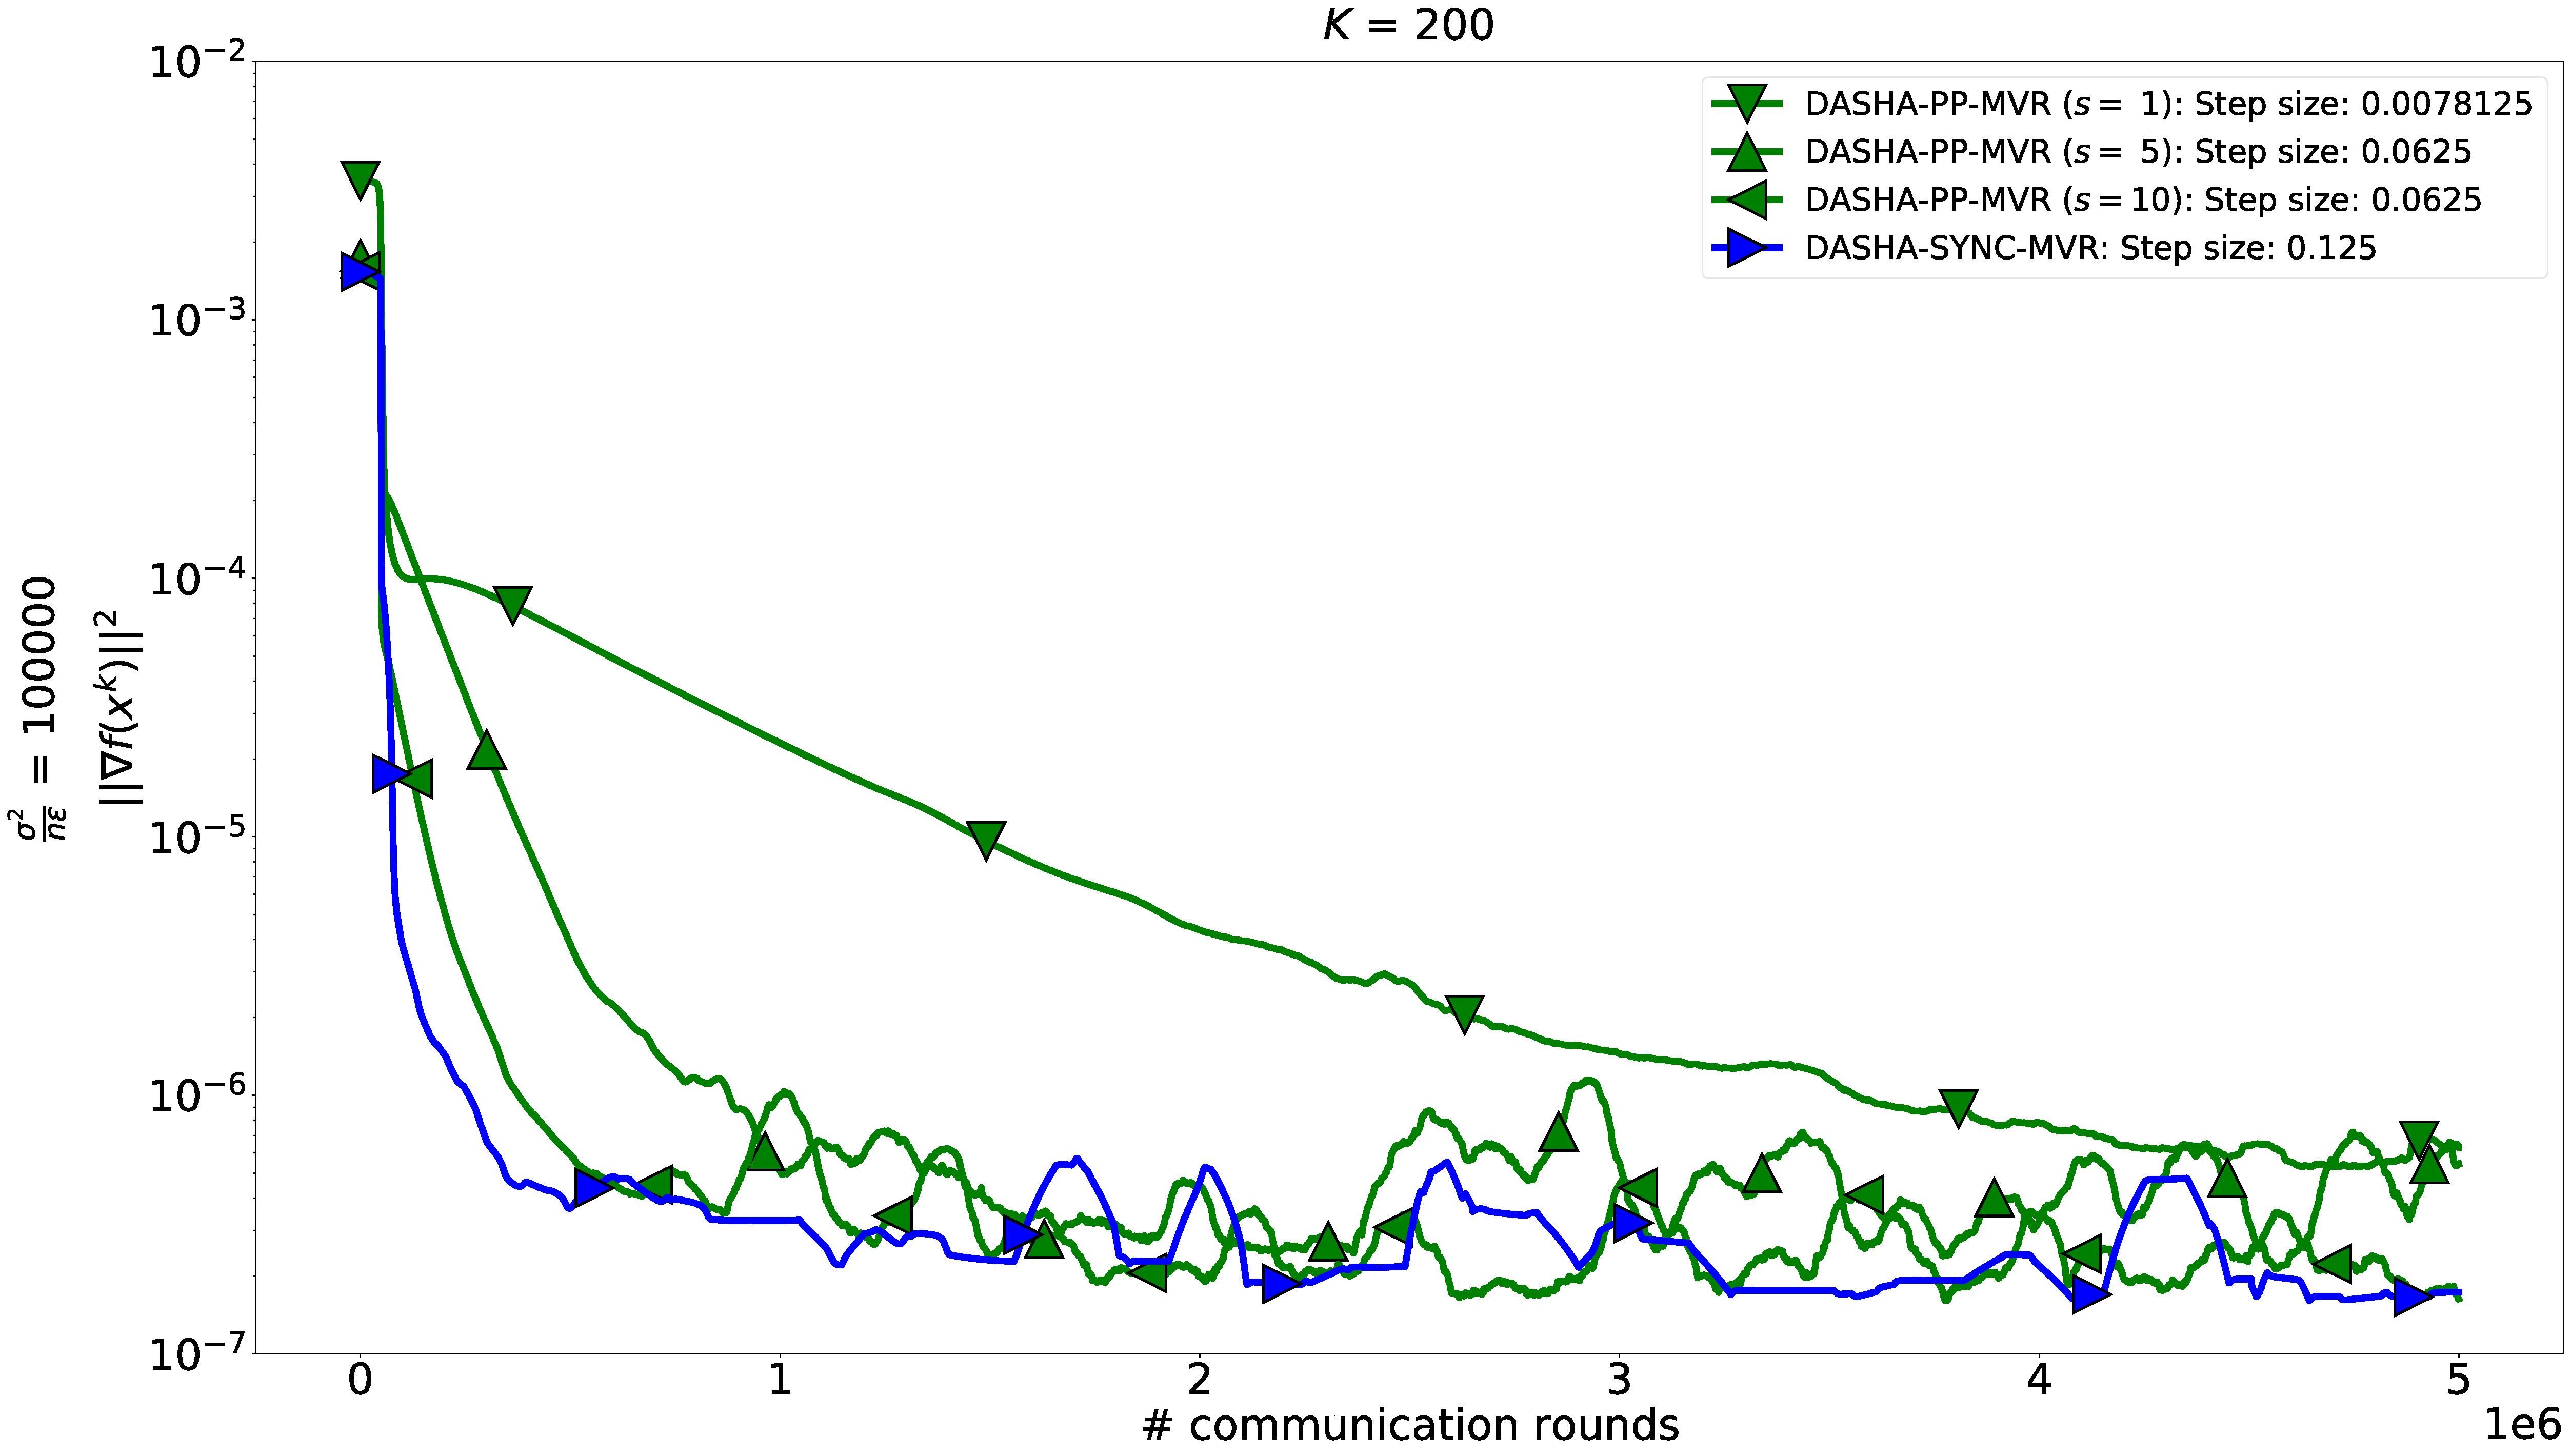
\includegraphics[width=0.75\linewidth]{experiments/neurips_2022_stochastic_real-sim_nof_200_numnodes_10_probs_mega_batch_100000_fix_nm_bug_longer.pdf}
%   \begin{tikzpicture}
%     \node[anchor=south west,inner sep=0] at (0,0) {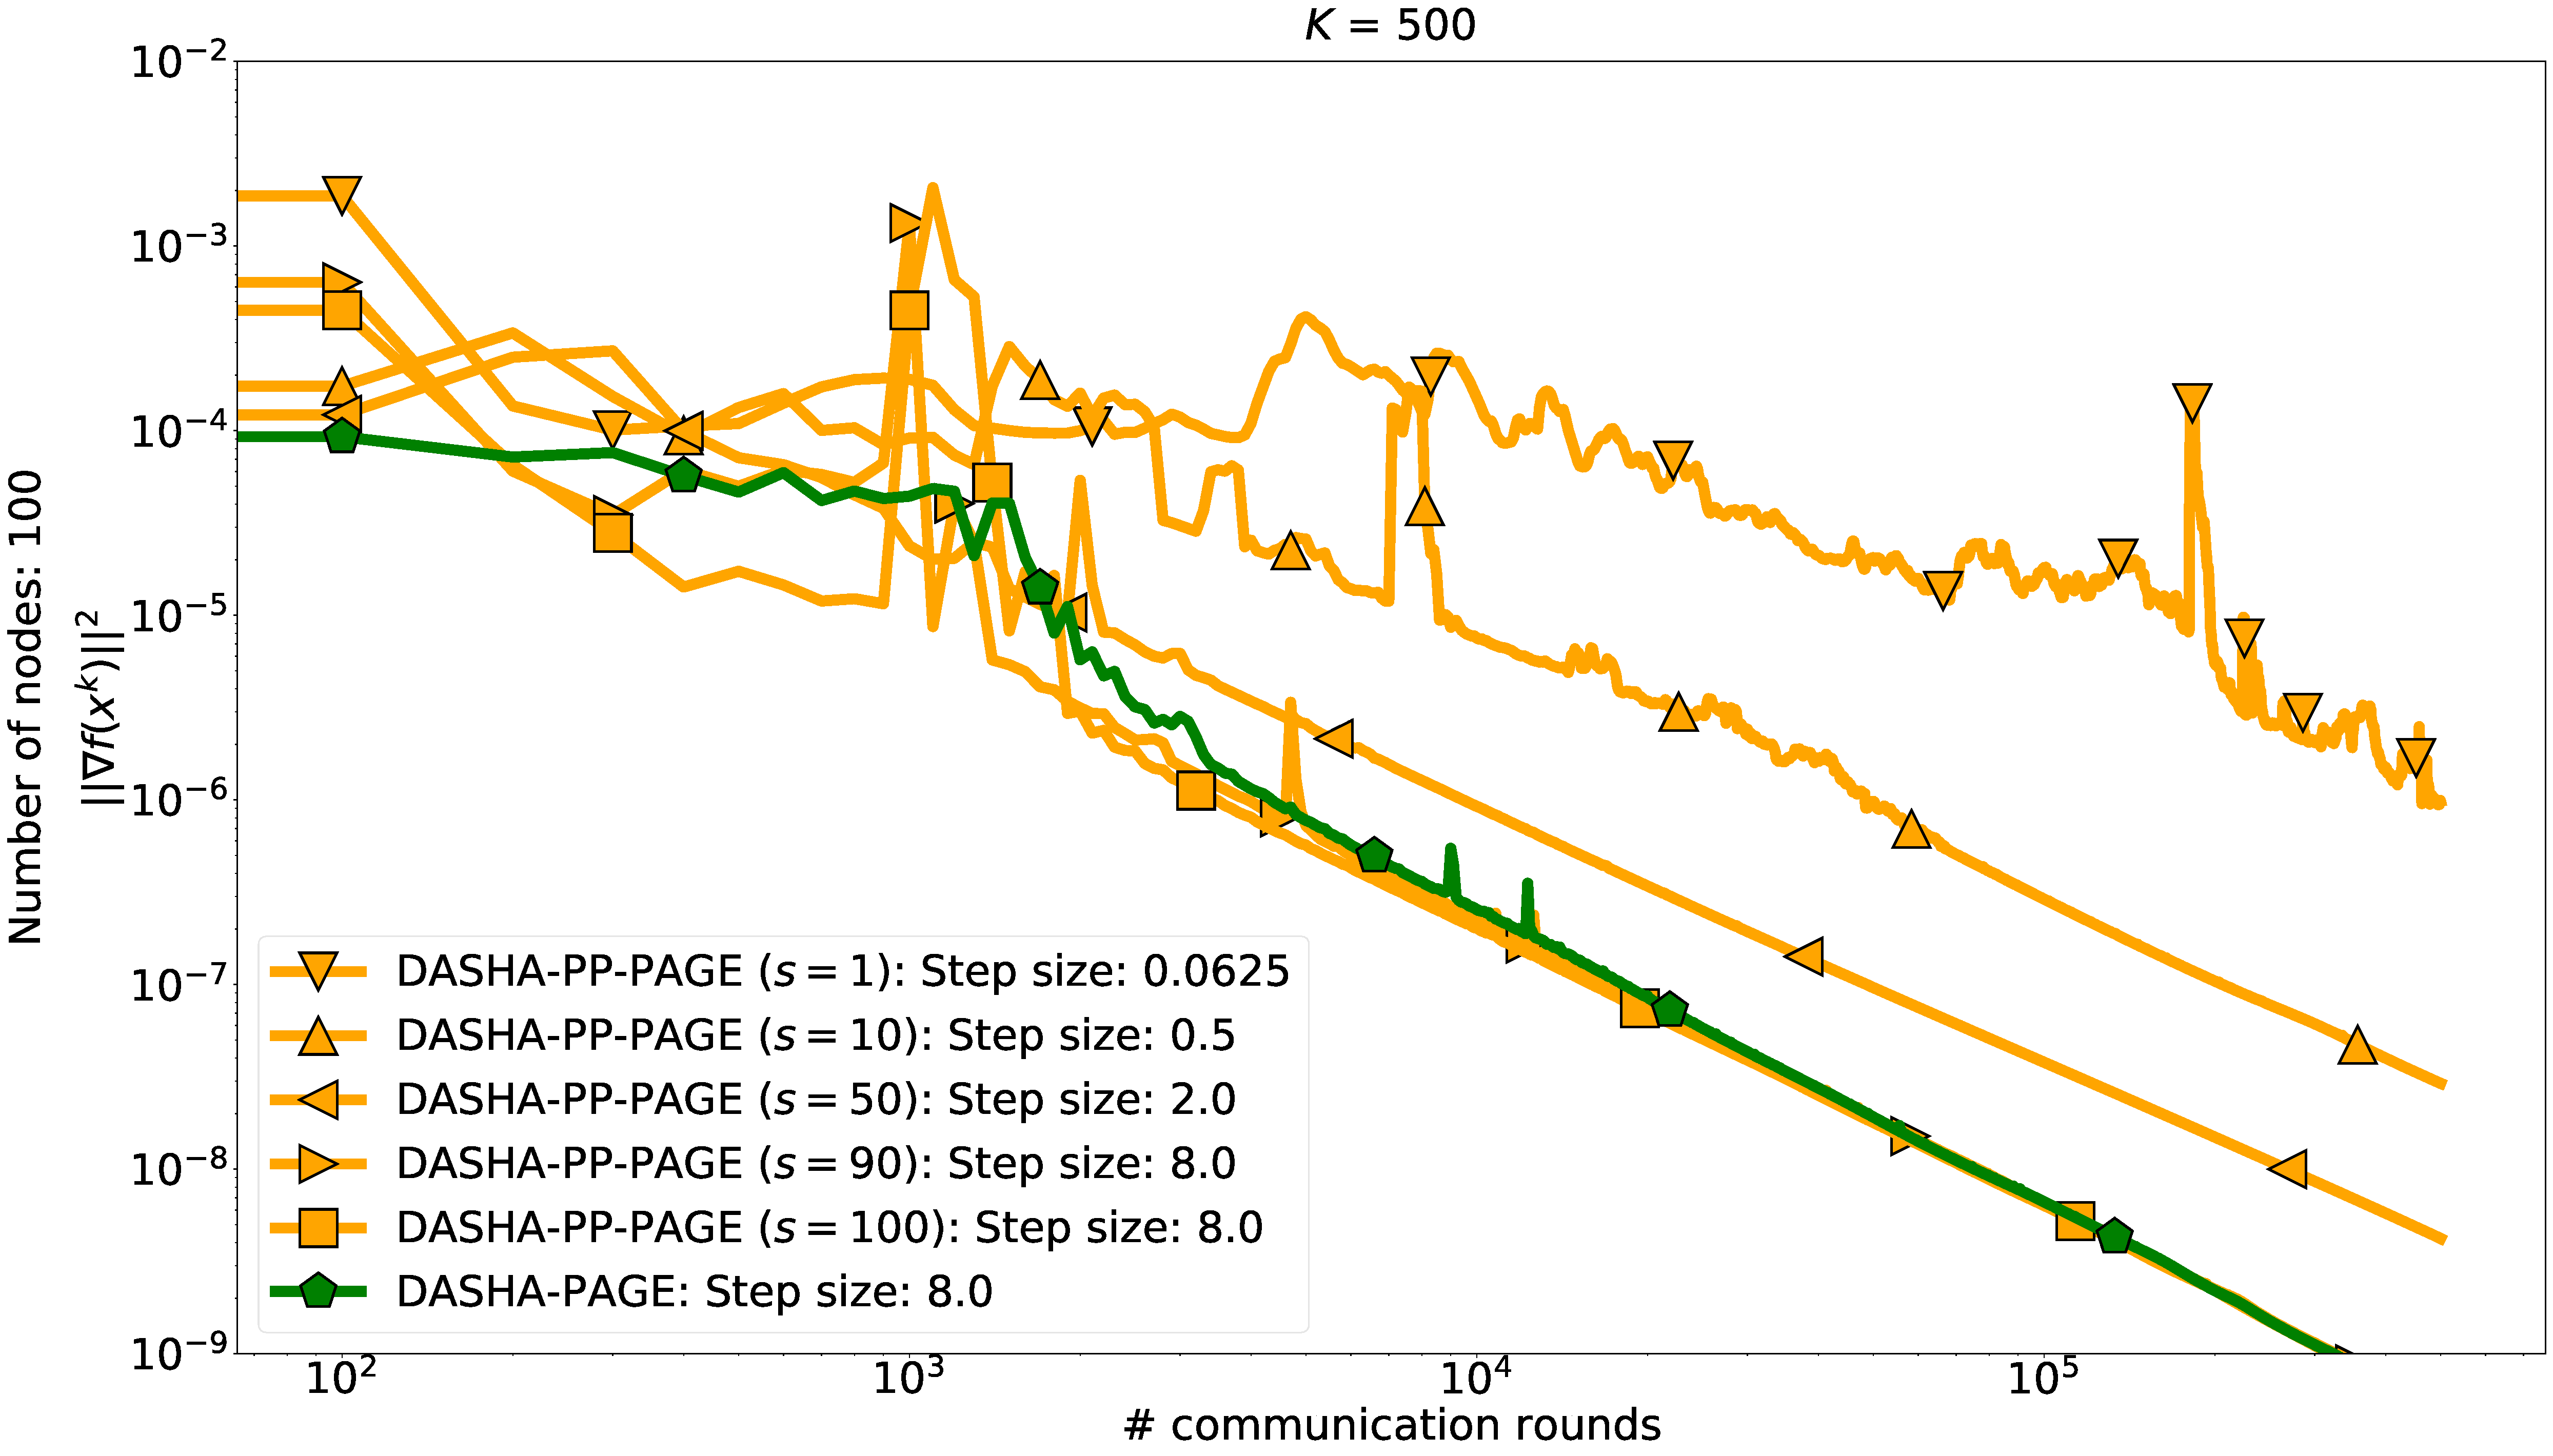
\includegraphics[width=\textwidth]{experiments/neurips_2022_finite_sum_real-sim_nof_500_numnodes_100_more_probs_batch_size_1_longer.pdf}};
%     \draw [black,ultra thick,decorate,decoration={brace,amplitude=20pt,raise=4ex}]
%       (7.0,3.0) -- (13.3,3.0) node[midway,yshift=+4.5em,xshift=+2em]{$\approx \times 100 \textnormal{ slower with } \probavailable = 0.01$};
%     \draw [black,ultra thick,decorate,decoration={brace,amplitude=20pt,raise=4ex}]
%       (9.8,1.5) -- (13.3,1.5) node[midway,yshift=+4.5em,xshift=+1em]{$\approx \times 10 \textnormal{ slower with } \probavailable = 0.1$};
%   \end{tikzpicture}
%   \caption{Classification task with the real-sim dataset, $K = 500$ in Rand$K$, in the finite-sum setting.}
%   \label{fig:real_sim_finite_sum}
% \end{figure}

% \begin{figure}[h]
%   \centering
%   % 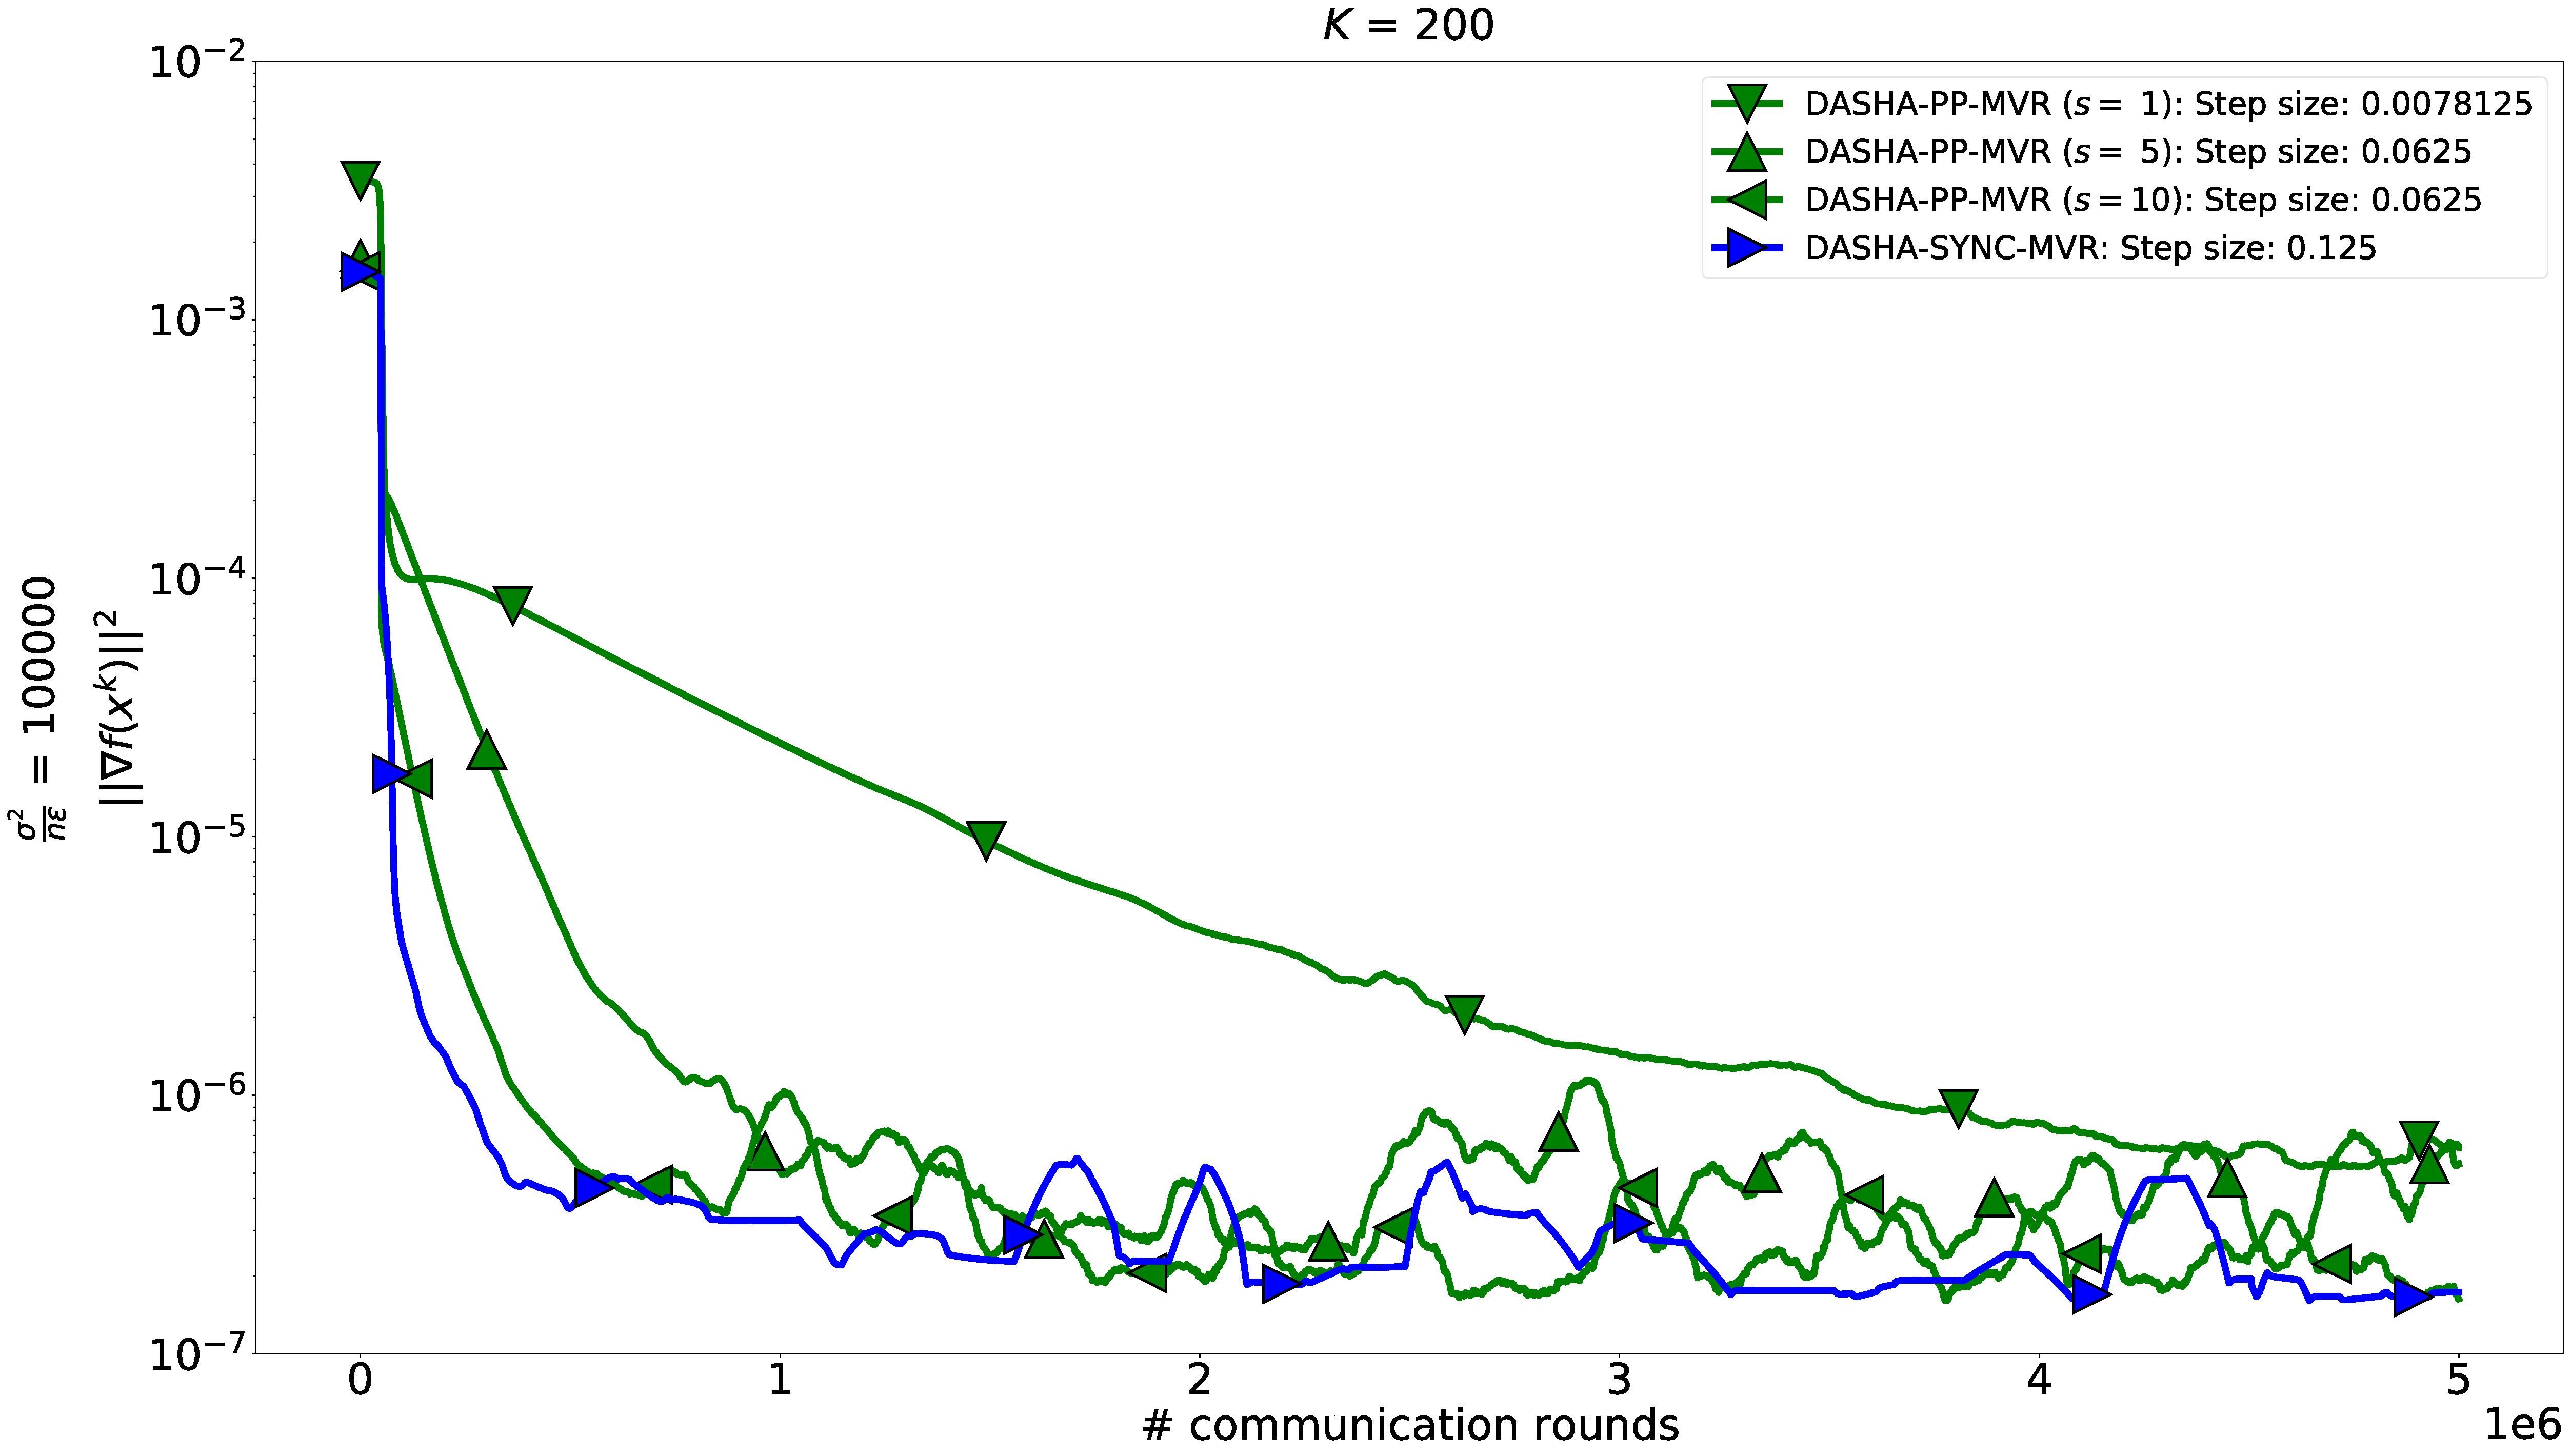
\includegraphics[width=0.75\linewidth]{experiments/neurips_2022_stochastic_real-sim_nof_200_numnodes_10_probs_mega_batch_100000_fix_nm_bug_longer.pdf}
%   \begin{tikzpicture}
%     \node[anchor=south west,inner sep=0] at (0,0) {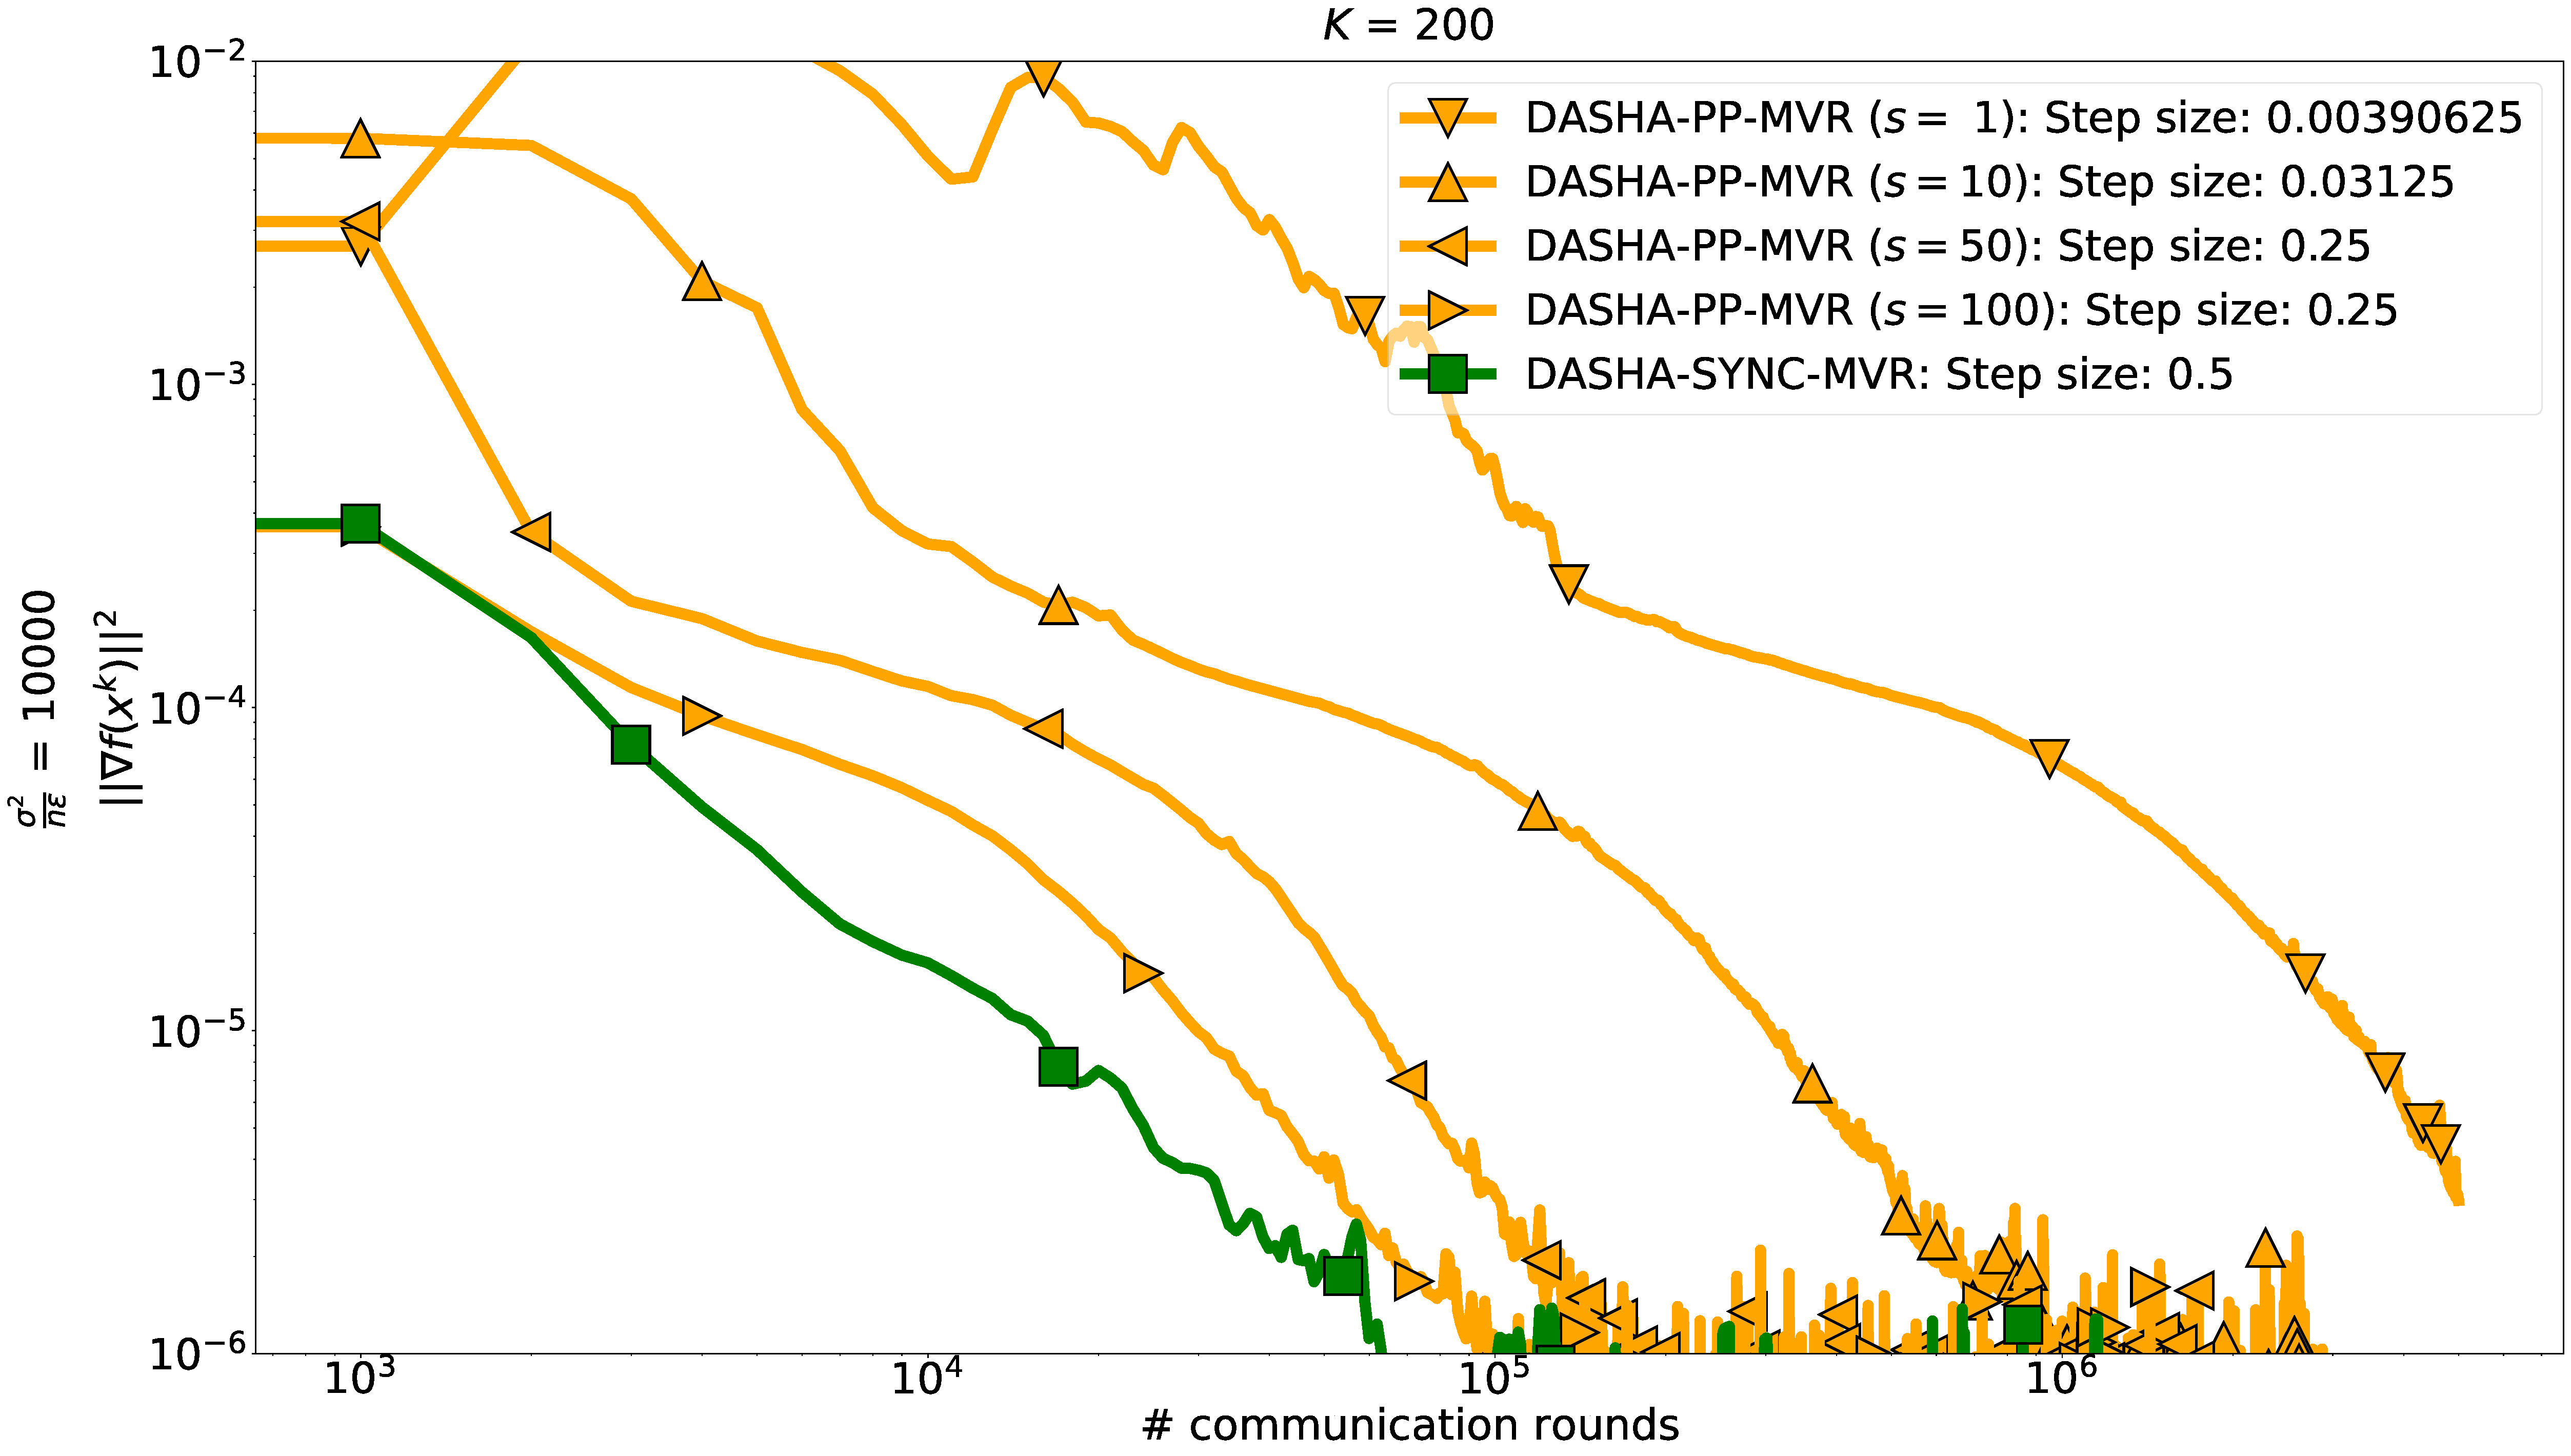
\includegraphics[width=\textwidth]{experiments/neurips_2022_stochastic_real-sim_nof_200_numnodes_100_probs_mega_batch_10000_fix_nm_bug_longer.pdf}};
%     \draw [black,ultra thick,decorate,decoration={brace,amplitude=20pt,raise=4ex}]
%       (7.3,0.8) -- (13.3,0.8) node[midway,yshift=+4.5em,xshift=+2em]{$\approx \times 100 \textnormal{ slower with } \probavailable = 0.01$};
%   \end{tikzpicture}
%   \caption{Classification task with the real-sim dataset, $\nicefrac{\sigma^2}{n \varepsilon B} = ?,$ and $K = 200$ in Rand$K$ in the stochastic setting.}
%   \label{fig:real_sim_stochastic}
% \end{figure}

\begin{figure}[h]
\centering
\begin{subfigure}{.5\textwidth}
  \centering
  \begin{tikzpicture}
    \node[anchor=south west,inner sep=0] at (0,0) {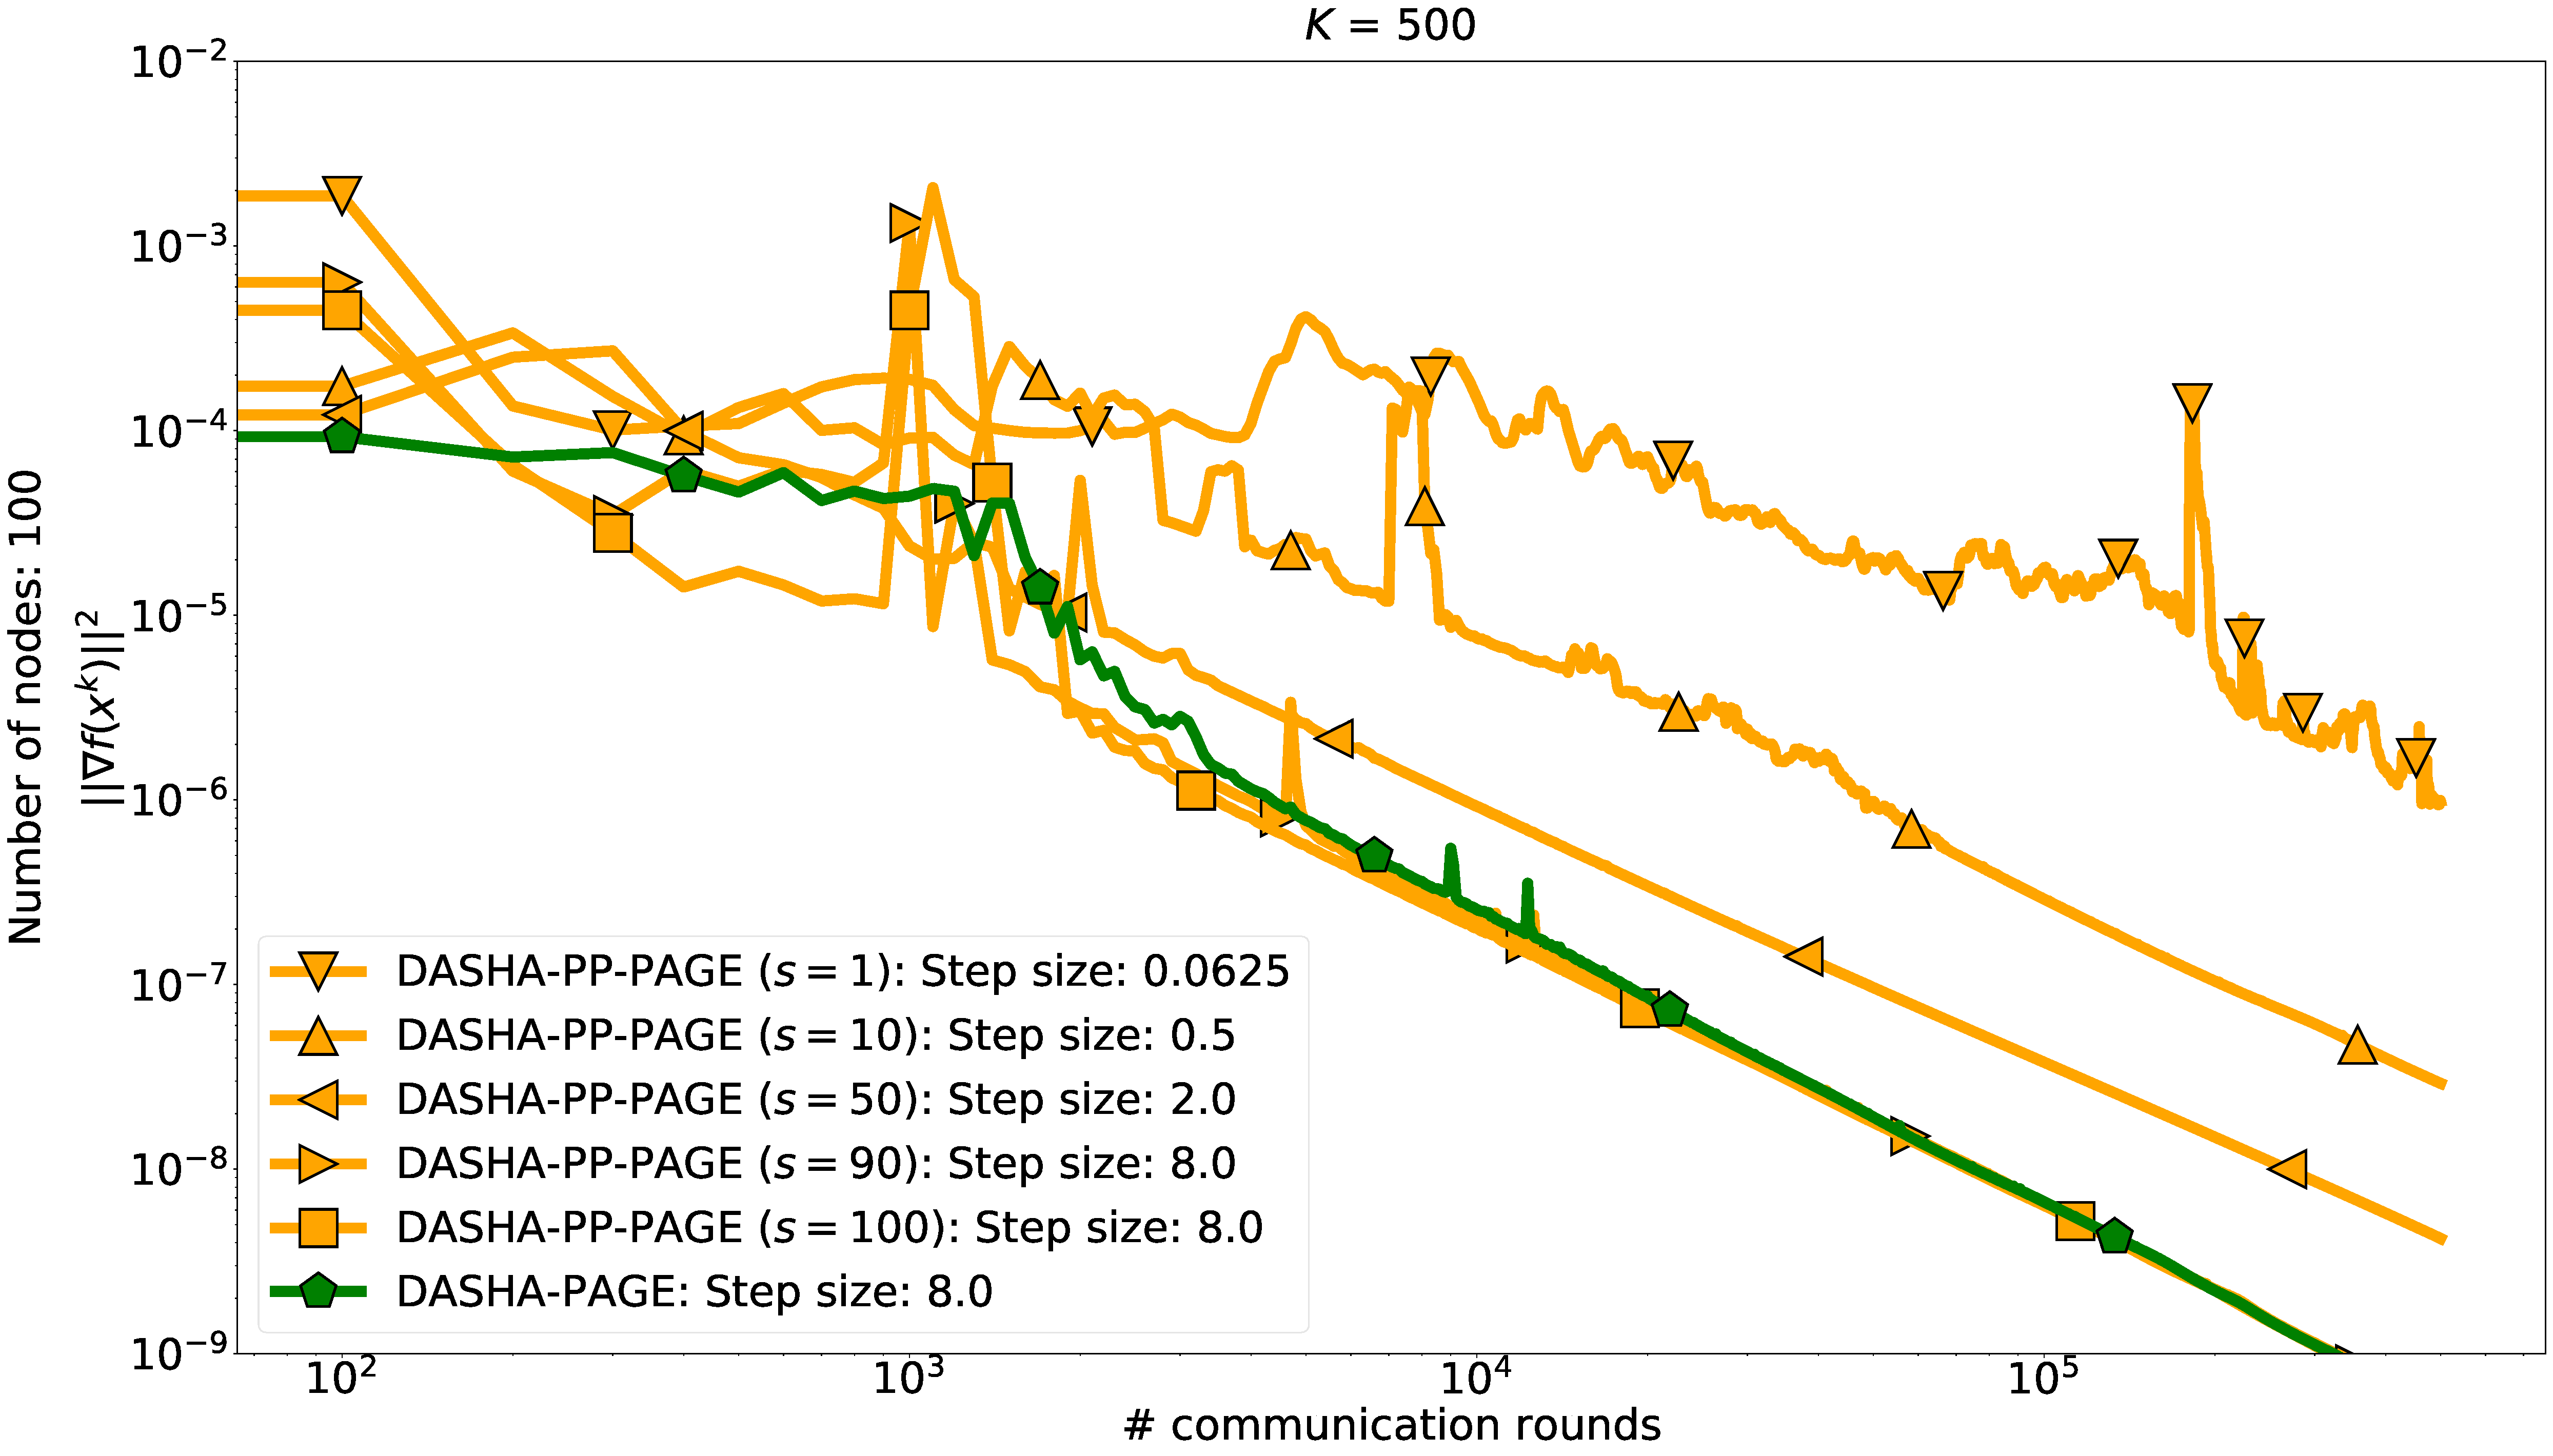
\includegraphics[width=\textwidth]{experiments/neurips_2022_finite_sum_real-sim_nof_500_numnodes_100_more_probs_batch_size_1_longer.pdf}};
    \draw [black,thick,<->] (3.6,1.8) -- (6.6,1.8) node[midway,yshift=-0.5em,xshift=+3.0em]{\scriptsize $\times 100 \textnormal{ slower}$};
    \draw [black,thick,<->] (5.1,1.0) -- (6.6,1.0) node[midway,yshift=-0.5em,xshift=-4.0em]{\scriptsize $\times 10 \textnormal{ slower}$};
    % \draw [black,ultra thick,decorate,decoration={brace,amplitude=20pt,raise=4ex}]
    %   (7.0,3.0) -- (13.3,3.0) node[midway,yshift=+4.5em,xshift=+2em]{$\approx \times 100 \textnormal{ slower with } \probavailable = 0.01$};
    % \draw [black,ultra thick,decorate,decoration={brace,amplitude=20pt,raise=4ex}]
    %   (9.8,1.5) -- (13.3,1.5) node[midway,yshift=+4.5em,xshift=+1em]{$\approx \times 10 \textnormal{ slower with } \probavailable = 0.1$};
  \end{tikzpicture}
  \caption{Finite-sum setting, $K = 500$ in Rand$K$.}
  \label{fig:real_sim_finite_sum}
\end{subfigure}\hfill
\begin{subfigure}{.5\textwidth}
  \centering
  \vspace{0.3cm}
  % 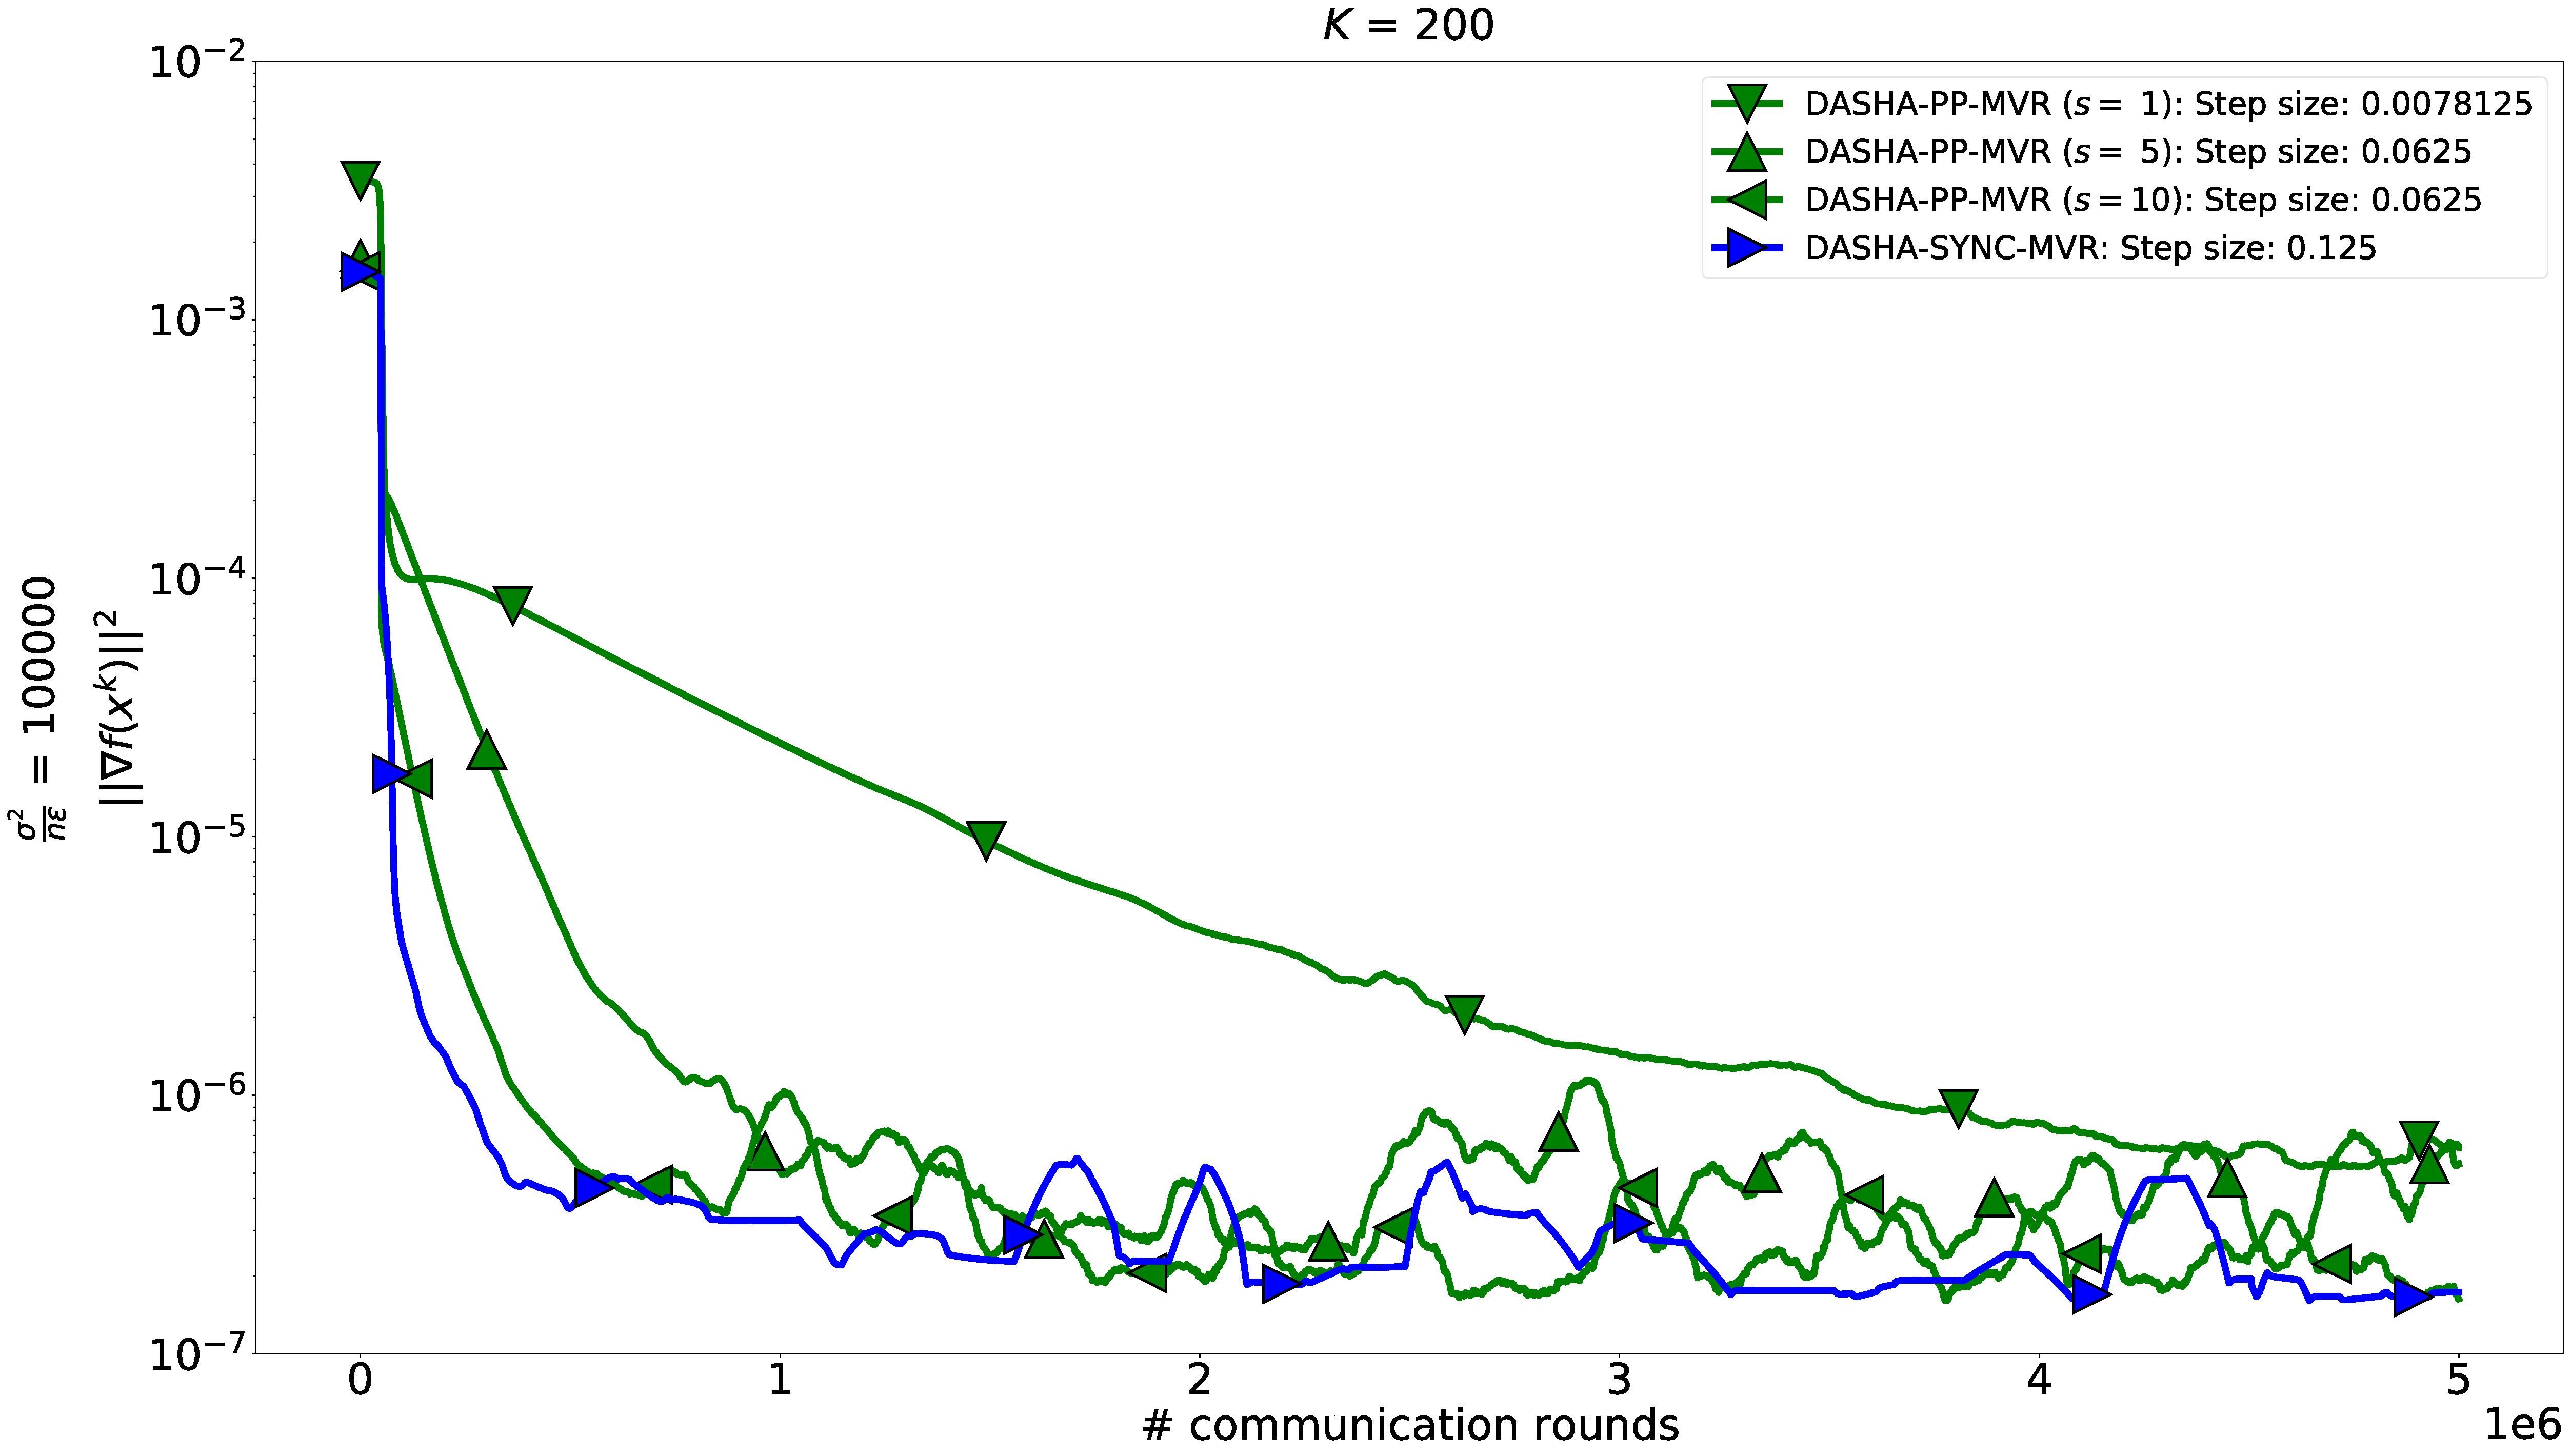
\includegraphics[width=0.75\linewidth]{experiments/neurips_2022_stochastic_real-sim_nof_200_numnodes_10_probs_mega_batch_100000_fix_nm_bug_longer.pdf}
  \begin{tikzpicture}
    \node[anchor=south west,inner sep=0] at (0,0) {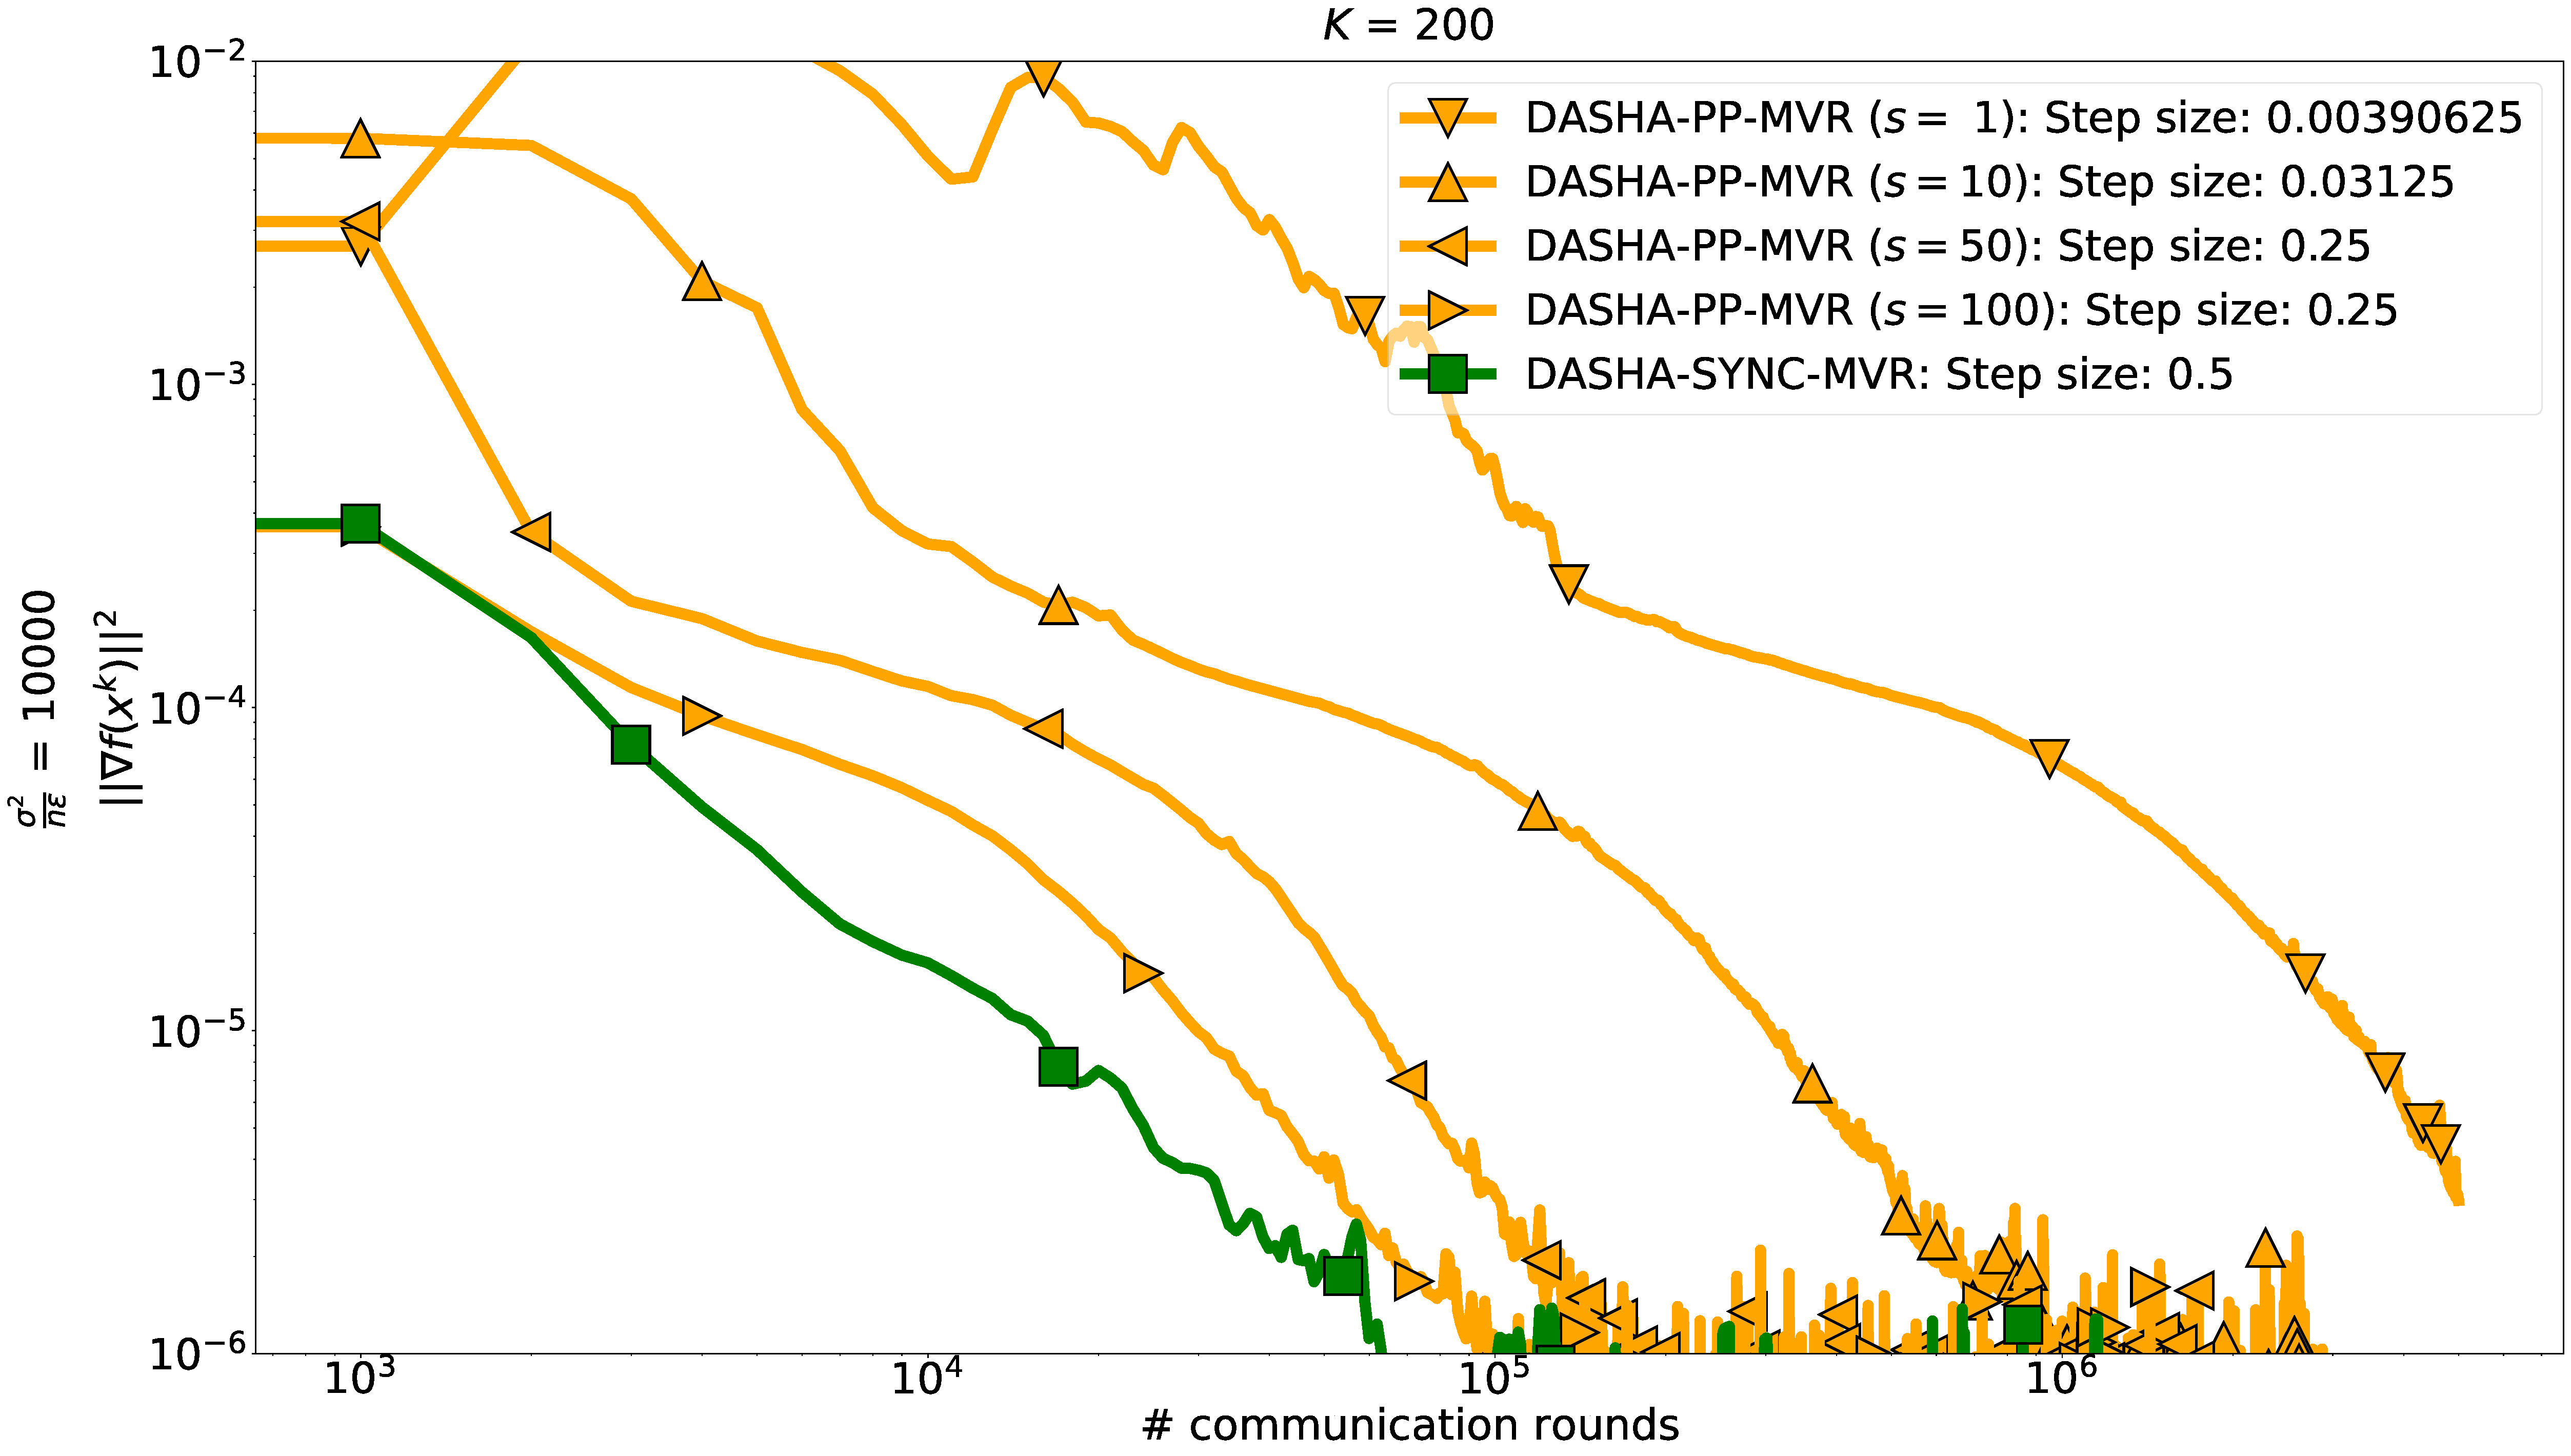
\includegraphics[width=\textwidth]{experiments/neurips_2022_stochastic_real-sim_nof_200_numnodes_100_probs_mega_batch_10000_fix_nm_bug_longer.pdf}};
    \draw [black,thick,<->] (3.7,0.7) -- (6.7,0.7) node[midway,yshift=+0.5em,xshift=+1.9em]{\scriptsize $\times 100 \textnormal{ slower}$};
    \draw [black,thick,<->] (3.7,0.8) -- (5.2,0.8) node[midway,yshift=+0.5em,xshift=+0.2em]{\scriptsize $\times 10 \textnormal{ slower}$};
    % \draw [black,ultra thick,decorate,decoration={brace,amplitude=20pt,raise=4ex}]
    %   (7.3,0.8) -- (13.3,0.8) node[midway,yshift=+4.5em,xshift=+2em]{$\approx \times 100 \textnormal{ slower with } \probavailable = 0.01$};
  \end{tikzpicture}
  \caption{Stochastic setting, $\nicefrac{\sigma^2}{n \varepsilon B} = 10000,$ and $K = 200$ in Rand$K$.}
  \label{fig:real_sim_stochastic}
\end{subfigure}
\caption{Classification task with the \textit{real-sim} dataset.}
\label{fig:test}
\end{figure}

\bibliographystyle{apalike}
\bibliography{sample_paper}

\end{document}
